% =================================================================================================
% Overview report: the Roman + Rubin joint microlensing forecast -- how the simulation works, what
% analyses are run on it and what each tells us, the numerical and physical results of the
% post-extinction-fix production runs (2026-09-24/25), and the next steps.
%
% Written for a scientific reader rather than a developer (restructured 2026-09-28 at the user's
% request; renamed from Report/onboarding/ the same day): no code history, no build or
% reproduction instructions in the PDF, and the text never says who it is written for. Provenance
% of every number is kept in comments beside the table or paragraph that quotes it, so the source
% still traces each one to a script's output file. Report/postfix/ is the short results report on
% the same runs and stays as it is.
%
% Build:  cd Report/overview && latexmk -pdf overview_report.tex
%         grep -c '^TODO:' overview_report.log      # must print 0
% GENERATED inputs (regenerate, do not edit; run from the repo root):
%   sample_table.tex  <- Report/overview/make_sample_table.py  (figures/samples/*/*/*_params.dat)
%   timeline.tex      <- Report/overview/make_timeline.py      (Baseline/{Bulge,Roman}Baseline.dat)
% Production runs: runs/prod_{bulge,bh,ns}_20260924, commit a5028fe, flags
%   --events 300 --lenses 50 --stride-roman 5 --pair-satellite (seed 42).
% Analysis: runs/yields_20260925.sh (y1, y3); figures/prod_20260925/run_p67.sh (p6, p7);
%   figures/wp_20260926/run_wp.sh (f2, f3, f4, h3, h5); analysis/y2_ss23_compare.py (y2).
% Next-steps costs: OPEN_ITEMS "The simulator cannot yet be split safely across cluster jobs".
% =================================================================================================
\documentclass[english,10pt,a4paper]{article}
\usepackage[T1]{fontenc}
\usepackage[margin=2.2cm]{geometry}
\usepackage{graphicx}
\graphicspath{{./}{../../figures/wp_20260926/}{../../figures/prod_20260925/}%
              {../../figures/yield_20260925/y3/}{../../figures/samples/}}
\usepackage{mathtools}
\usepackage{amssymb}
\usepackage{booktabs}
\usepackage{longtable}
\usepackage{array}
\usepackage{xcolor}
\usepackage{tikz}
\usetikzlibrary{positioning,arrows.meta,calc}
\usepackage[colorlinks=true,allcolors=blue]{hyperref}
\usepackage{caption}
\usepackage{subcaption}
\usepackage[authoryear,round]{natbib}
\usepackage[section]{placeins}
\usepackage{enumitem}
\setlist{itemsep=2pt,topsep=3pt}
\setlength{\emergencystretch}{3em}

\newcommand{\tE}{t_{\rm E}}
\newcommand{\piE}{\pi_{\rm E}}
\newcommand{\tetE}{\theta_{\rm E}}
\newcommand{\Ml}{M_{\rm L}}
\newcommand{\Msun}{M_\odot}
\newcommand{\Neff}{N_{\rm eff}}
\newcommand{\code}[1]{\texttt{#1}}
\makeatletter
\newcommand{\sampletable}{\@@input sample_table.tex }
\newcommand{\surveytimeline}{\@@input timeline.tex }
\makeatother
\newcommand{\TODO}[1]{\textcolor{red}{\textbf{[TODO: #1]}}\typeout{TODO: #1}}

% Flowchart styles.
\tikzset{
  every picture/.append style={>={Stealth[length=2mm]}},
  box/.style={draw=black!55, rounded corners=2pt, align=center, font=\footnotesize,
              inner sep=3pt, fill=blue!5},
  inbox/.style={box, fill=orange!10, text width=2.8cm, minimum height=2.3cm},
  ask/.style={draw=black!55, align=center, font=\footnotesize, inner sep=3pt, fill=yellow!18},
  side/.style={box, fill=black!4, text width=3.6cm},
  arr/.style={->, thick, black!65},
  lab/.style={font=\scriptsize\itshape, black!70},
}

% One sample event on its own page. #1 = path under figures/samples/, #2 = caption, #3 = label.
\newcommand{\samplefig}[3]{%
\begin{figure}[p]
\centering
\includegraphics[height=0.86\textheight,width=\textwidth,keepaspectratio]{#1}
\caption{#2}
\label{#3}
\end{figure}}

\title{Microlensing toward the Galactic bulge with Roman and Rubin:\\
       how the forecast is made, what it measures, and what it finds}
\author{Ali Salehi}
\date{\today}

\begin{document}
\maketitle

% Numbers: figures/yield_20260925/y3/y3_coefficients.md (N_1, footprint and whole scan, per object);
% figures/u1_20260929/u1_numbers.md (every error bar; Roman-for-Rubin; dust; shares; shifts);
% figures/u1_20260929/u2_resolution_depth.csv (image resolution at Roman's 5-sigma depth);
% extinctiontest (A_r/A_V 0.854, A_F146/A_V 0.197 at R_V = 2.5).
% ABSTRACT NUMBERS ARE DUST-CORRECTED: figures/u1_20260929/u5_corrected_numbers.md (total error =
% Monte Carlo (+) correction systematic; Deviation 63); real-layout factor from
% u4_dust_check_hybrid.csv Part 2.
\begin{abstract}
We forecast which microlensing events toward the Galactic bulge will be detected by the Nancy Grace
Roman Space Telescope's Galactic Bulge Time Domain Survey and by the Vera C.\ Rubin Observatory's
Legacy Survey of Space and Time, and how precisely each survey, and the two together, will measure
them, for three lens populations: ordinary stars and stellar remnants, isolated black holes, and
neutron stars. The simulation's dust is too thin near the Galactic plane; every number below is
corrected for it unless stated, and its uncertainty combines the Monte Carlo error with the correction's own
systematic error (Section~\ref{sec:dust}). Over the decade 2026--2036, inside Roman's footprint
($1.47$\,deg$^2$ as modelled), Roman is expected to detect $(5.04\pm0.29)\times10^4$ events by ordinary
lenses and to measure $830\pm110$ of their lens masses to $10\%$; Rubin detects
$(4.9\pm0.5)\times10^3$ there and $(7.8\pm1.2)\times10^4$ across the $59$\,deg$^2$ of bulge simulated.
Compact-object yields scale with the fraction $F$ of the Galaxy's stellar mass the population holds.
Roman detects $(5{,}660\pm320)\,F$ black-hole events ($3$--$1000\,\Msun$), i.e.\ $28$--$170$ for
$F=0.005$--$0.03$, with $3$--$17$ masses measured to $10\%$; and $(36{,}500\pm2{,}300)\,F$ neutron-star
events, i.e.\ $180$--$2{,}190$ for $F=0.005$--$0.06$, with $6$--$66$ masses. The adopted GBTDS layout,
which the simulated footprint does not follow exactly, would add roughly $15$--$24\%$ to Roman's
yields. Inside its footprint Roman dominates, above all because of dust: at the median extinction of
Roman's footprint detections, $A_V=7.2\pm0.3$, Rubin's $r$-band source is dimmed by $6.1$\,mag and
Roman's F146 source by only $1.4$\,mag, and Roman detects eight to ten times as many events there. Rubin
therefore changes Roman's precision on shared events by less than $0.4\%$ (median) and adds at
most $9$--$13\%$ to the number of $10\%$ masses. \textbf{The gain in the other direction is far larger.}
For the events Rubin detects inside the footprint, adding Roman's data sharpens the timescale a
median $8$--$17$-fold, raises the fraction with both timescale and parallax measured from $5$--$12\%$
to $28$--$83\%$, and turns lens masses to $10\%$ from essentially none into $(8.1\pm1.5)\%$ of them for
ordinary lenses, $(15.7\pm1.2)\%$ for neutron stars and $(53.3\pm1.8)\%$ for black holes. Rubin's own
strengths are sky area, with $(59\pm5)\%$ of all detections outside Roman's footprint, and short
events that fall wholly inside Roman's season gaps, whose timescale precision it improves by an order
of magnitude as simulated (not corrected for the dust, which can only reduce this gain). The Einstein radius, and so the mass, is Roman's astrometric measurement. Black-hole
centroid shifts (median $3.39\pm0.04$\,mas among Roman's detections) exceed a single exposure's
precision; ordinary-lens shifts (median $0.123\pm0.002$\,mas)
emerge only by averaging $\sim\!5\times10^4$ exposures, which assumes that Roman's $1.1$\,mas
astrometric floor averages down, the largest remaining uncertainty in these results. Heavy lenses can
also split the source into two images that a telescope resolves. With the criterion of
\citet{SajadianMakler2026}, Roman could separate them in $(34.2\pm1.2)\%$ of its black-hole detections
if a separation of five times the astrometric error suffices, $(15.3\pm0.9)\%$ at twenty times, and
$(0.25\pm0.04)\%$ if the width of its point-spread function is required; for neutron stars and
ordinary lenses the most permissive figures are $(1.7\pm0.2)\%$ and $(0.8\pm0.3)\%$. Rubin resolves
the images of about $5\%$ of the black-hole events it detects (a figure not corrected for the dust)
and of essentially no others.
\end{abstract}

\tableofcontents
\clearpage

% =================================================================================================
\section{The science question}
\label{sec:science}

\subsection{Microlensing and the mass of a dark lens}
When a foreground star (the \emph{lens}, mass $\Ml$ at distance $D_L$) passes close to the line of
sight to a background star (the \emph{source}, at $D_S$), its gravity bends the source's light into
two unresolved images and magnifies it. The natural angular scale is the Einstein radius
\begin{equation}
\tetE = \sqrt{\kappa\,\Ml\,\pi_{\rm rel}},\qquad \kappa = 8.144\,{\rm mas}\,\Msun^{-1},\qquad
\pi_{\rm rel} = {\rm AU}\,(1/D_L - 1/D_S),
\end{equation}
typically a fraction of a milliarcsecond (mas) for a bulge star and several mas for a nearby black
hole. With the lens--source separation $u$ in units of $\tetE$, the point-lens magnification is
\citep{Paczynski1986}
\begin{equation}
A(u) = \frac{u^2+2}{u\sqrt{u^2+4}},\qquad u(t) = \sqrt{u_0^2 + \bigl((t-t_0)/\tE\bigr)^2},
\end{equation}
where $u_0$ is the impact parameter, $t_0$ the time of closest approach and $\tE = \tetE/\mu_{\rm rel}$
the \emph{Einstein timescale}. The timescale is the one physical quantity a simple light curve gives,
and it mixes mass, distance and velocity, so a light curve alone does not give the lens mass. Two more
observables are needed (Fig.~\ref{fig:observables}):
\begin{itemize}
\item the \emph{microlens parallax} $\piE = \pi_{\rm rel}/\tetE$, measured from the distortion of
      the light curve as the observer moves (annual parallax, from Earth's orbit) or from two observers
      at once (satellite parallax: here Roman at L2 and Rubin on the ground, $0.01$\,AU apart);
\item the Einstein radius $\tetE$ itself, measured from the \emph{astrometric} shift of the
      light centroid, $\delta\theta = \tetE\,u/(u^2+2)$, which peaks at $\tetE/\sqrt8$ when
      $u=\sqrt2$.
\end{itemize}
Then $\Ml = \tetE/(\kappa\piE)$ \citep{Gould2000Formalism}. Measuring the masses of \emph{dark}
lenses -- isolated black holes and neutron stars -- is the main reason to want both observables.
Ordinary bulge events have $\tE\sim 20$\,d; black-hole events last hundreds of days.

A third, more direct route to $\tetE$ exists for heavy, nearby lenses: seeing the two images
themselves. They lie on either side of the lens, separated by
\begin{equation}
\Delta\theta = \tetE\sqrt{u^2+4}\;\ge\;2\,\tetE,
\end{equation}
so a black hole of tens of solar masses a few kpc away splits its source by $\gtrsim10$\,mas. The
difficulty is that the separation is smallest when both images are bright, at closest approach,
and grows only as the fainter (minor) image fades, with magnification
$A_- = (u^2+2)/(2u\sqrt{u^2+4})-\tfrac12\to1/u^4$. Section~\ref{sec:resolve} asks how often each
telescope could tell the two apart.

\begin{figure}[h]
\centering
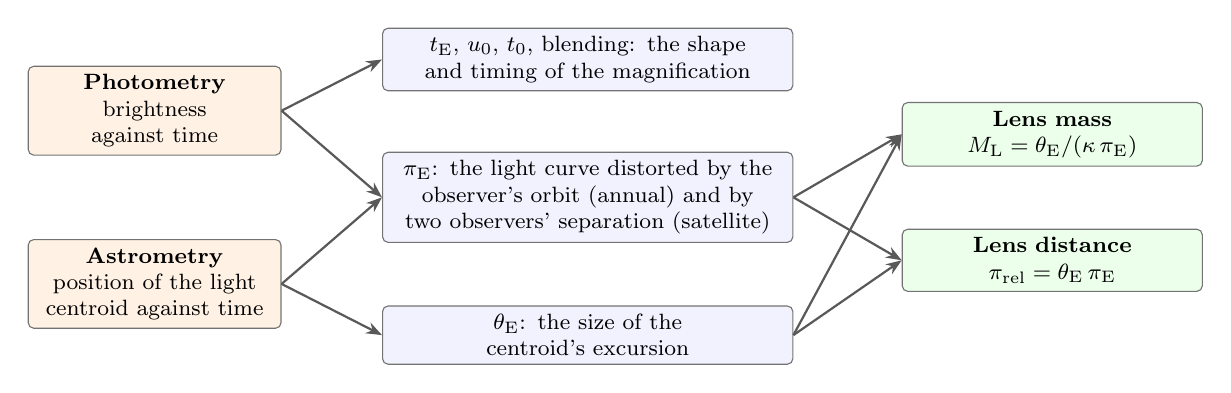
\begin{tikzpicture}
\node[box, fill=orange!10, text width=3.0cm] (phot) at (0,1.1)
  {\textbf{Photometry}\\ brightness against time};
\node[box, fill=orange!10, text width=3.0cm] (ast) at (0,-1.1)
  {\textbf{Astrometry}\\ position of the light centroid against time};
\node[box, text width=5.0cm] (te) at (5.5,1.75)
  {$\tE$, $u_0$, $t_0$, blending: the shape and timing of the magnification};
\node[box, text width=5.0cm] (pie) at (5.5,0)
  {$\piE$: the light curve distorted by the observer's orbit (annual) and by two observers'
   separation (satellite)};
\node[box, text width=5.0cm] (the) at (5.5,-1.75)
  {$\tetE$: the size of the centroid's excursion};
\node[box, fill=green!8, text width=3.6cm] (mass) at (11.4,0.8)
  {\textbf{Lens mass}\\ ${\Ml = \tetE/(\kappa\,\piE)}$};
\node[box, fill=green!8, text width=3.6cm] (dist) at (11.4,-0.8)
  {\textbf{Lens distance}\\ ${\pi_{\rm rel} = \tetE\,\piE}$};
\draw[arr] (phot.east) -- (te.west);
\draw[arr] (phot.east) -- (pie.west);
\draw[arr] (ast.east) -- (pie.west);
\draw[arr] (ast.east) -- (the.west);
\draw[arr] (pie.east) -- (mass.west);
\draw[arr] (the.east) -- (mass.west);
\draw[arr] (pie.east) -- (dist.west);
\draw[arr] (the.east) -- (dist.west);
\end{tikzpicture}
\caption{From observables to a lens mass. A light curve alone gives the timescale; the mass needs the
parallax $\piE$ and the Einstein radius $\tetE$, and their fractional errors add in quadrature,
$(\sigma_M/M)^2 = (\sigma_{\piE}/\piE)^2 + (\sigma_{\tetE}/\tetE)^2$.}
\label{fig:observables}
\end{figure}

\subsection{Two surveys with complementary strengths}
\begin{itemize}
\item \textbf{Roman's Galactic Bulge Time Domain Survey (GBTDS)} images six fields covering
      $\sim\!1.7$\,deg$^2$ ($1.47$\,deg$^2$ as modelled here; Section~\ref{sec:simulator}) in the
      near-infrared F146 filter. It observes only in ten seasons of
      $\sim\!70$ days, separated by $\sim\!110$-day gaps when the bulge is too close to the Sun:
      six high-cadence seasons (three at each end of the mission), in which every field is imaged
      every $12.1$ minutes, and four low-cadence seasons in between, with one visit every five days
      \citep{STScIGBTDS}.
      Near-infrared light suffers little dust extinction, and Roman's diffraction-limited images
      give per-exposure astrometry at the $\sim\!1$\,mas level for bright stars
      \citep{Sanderson2019WFIRSTastrometry}.
\item \textbf{Rubin's Legacy Survey of Space and Time (LSST)} \citep{Ivezic2019LSST} observes a
      far larger area in six optical bands ($ugrizy$), every few days while the bulge is up, for ten
      years, from the ground; the optical bands are heavily extincted toward the bulge.
\end{itemize}
Fig.~\ref{fig:timeline} shows the two schedules at one sightline in Roman's footprint. The contrast
is stark: $\sim\!2{,}400$ Rubin visits spread over ten years, against $\sim\!5\times10^4$ Roman
exposures packed into six $70$-day seasons.

\begin{figure}[h]
\centering
\surveytimeline
\caption{The two surveys' observing windows at one sightline in Roman's footprint,
$(l,b)=(\tlL^\circ,\tlB^\circ)$. Orange: Rubin, $\tlNrub$ visits in six bands, drawn as windows
separated by more than $20$ days. Blue: Roman's ten seasons, $\tlNrom$ exposures in all; dark:
high cadence ($\sim\!8{,}200$--$8{,}600$ exposures per season), light: low cadence ($14$--$15$
exposures per season). The clock starts at Rubin's first bulge visit (2026-04-11). Roman's mission is
placed on 2028-04-10 to 2032-12-23; since its real start date is uncertain, this is a modelling
choice, and it leaves two years of Rubin-only data before Roman and three after.}
\label{fig:timeline}
\end{figure}

\textbf{The question:} which events does each survey detect, how well does each characterise them,
and what does the \emph{combination} buy? Two expectations motivated the joint study. Short events
that peak in Roman's gaps should be Rubin's or nobody's. Long events should need Rubin's decade of
coverage for the annual parallax that turns $\tE$ into a mass. The results below test both.

% =================================================================================================
\section{How the simulation works}
\label{sec:simulator}

The simulation is a Monte Carlo over the bulge sky (Fig.~\ref{fig:overview}). At each sky position it
draws many random source--lens pairs from a model of the Galaxy. For each pair it generates the data
each telescope would actually record, on the surveys' real schedules and with their noise. It then
decides whether each survey would detect the event, and forecasts how precisely each survey, and both
together, would measure it. It builds on Dr.\ Sajadian's simulation of microlensing toward the
Magellanic Clouds, the code lineage published with \citet{SajadianMakler2026}, extended to two
observatories.

\begin{figure}[h]
\centering
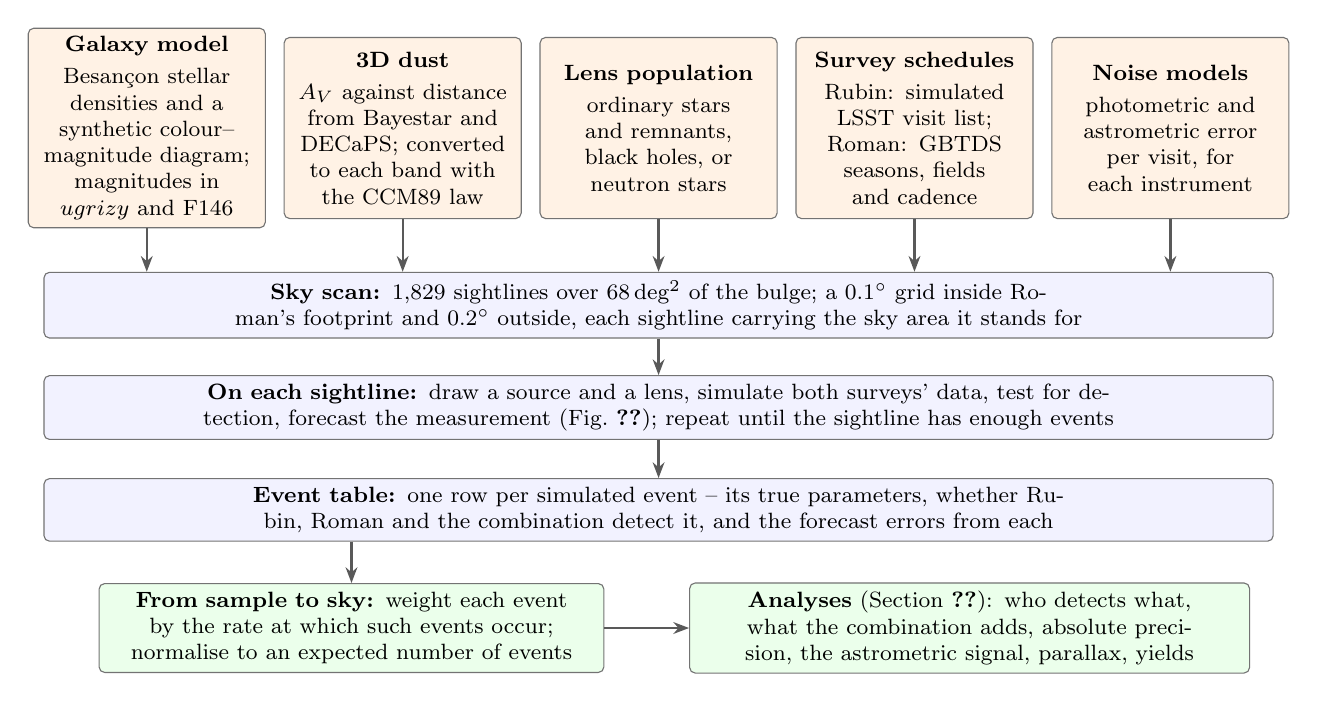
\begin{tikzpicture}
\node[inbox] (g) at (0,0)     {\textbf{Galaxy model}\\[2pt] Besan\c{c}on stellar densities and a
  synthetic colour--magnitude diagram; magnitudes in $ugrizy$ and F146};
\node[inbox] (d) at (3.25,0)  {\textbf{3D dust}\\[2pt] $A_V$ against distance from Bayestar and
  DECaPS; converted to each band with the CCM89 law};
\node[inbox] (p) at (6.5,0)   {\textbf{Lens population}\\[2pt] ordinary stars and remnants, black
  holes, or neutron stars};
\node[inbox] (s) at (9.75,0)  {\textbf{Survey schedules}\\[2pt] Rubin: simulated LSST visit list;
  Roman: GBTDS seasons, fields and cadence};
\node[inbox] (e) at (13.0,0)  {\textbf{Noise models}\\[2pt] photometric and astrometric error per
  visit, for each instrument};
\node[box, text width=15.4cm] (sky) at (6.5,-2.25)
  {\textbf{Sky scan:} $1{,}829$ sightlines over $68$\,deg$^2$ of the bulge; a $0.1^\circ$ grid inside
   Roman's footprint and $0.2^\circ$ outside, each sightline carrying the sky area it stands for};
\node[box, text width=15.4cm] (mc) at (6.5,-3.55)
  {\textbf{On each sightline:} draw a source and a lens, simulate both surveys' data, test for
   detection, forecast the measurement (Fig.~\ref{fig:event}); repeat until the sightline has enough
   events};
\node[box, text width=15.4cm] (tab) at (6.5,-4.85)
  {\textbf{Event table:} one row per simulated event -- its true parameters, whether Rubin, Roman
   and the combination detect it, and the forecast errors from each};
\node[box, fill=green!8, text width=6.2cm] (w) at (2.6,-6.35)
  {\textbf{From sample to sky:} weight each event by the rate at which such events occur;
   normalise to an expected number of events};
\node[box, fill=green!8, text width=6.9cm] (an) at (10.45,-6.35)
  {\textbf{Analyses} (Section~\ref{sec:analyses}): who detects what, what the combination adds,
   absolute precision, the astrometric signal, parallax, yields};
\foreach \n in {g,d,p,s,e} \draw[arr] (\n.south) -- (\n.south |- sky.north);
\draw[arr] (sky) -- (mc);
\draw[arr] (mc) -- (tab);
\draw[arr] (tab.south -| w.north) -- (w.north);
\draw[arr] (w.east) -- (an.west);
\end{tikzpicture}
\caption{The simulation from inputs to results. The upper half generates simulated events; the lower
half turns the simulated sample into statements about the real sky.}
\label{fig:overview}
\end{figure}

\subsection{The inputs}
\begin{description}[leftmargin=0pt,style=unboxed]
\item[The Galaxy.] Stellar densities of the thin and thick disc, bulge and halo along each sightline
  come from the Besan\c{c}on model \citep{Robin2003}, and source stars are drawn from its synthetic
  colour--magnitude diagram, with MIST bolometric corrections \citep{Choi2016MIST} giving magnitudes
  in Rubin's six bands and Roman's F146.
\item[Dust.] Three-dimensional maps \citep[Bayestar and DECaPS;][]{Green2019Bayestar,Zucker2025DECaPS} give $A_V$ as a
  function of distance along each sightline, and the \citet{Cardelli1989} law ($R_V=2.5$ in the
  bulge, $3.1$ elsewhere) converts it to each band: $A_r/A_V=0.85$ but $A_{\rm F146}/A_V=0.20$.
  Toward the bulge this single ratio decides much of the comparison between the two surveys. A
  declination rule gives almost all of Roman's footprint to Bayestar, which cannot see through the
  dust near the plane and there gives three to six times too little dust (Section~\ref{sec:dust}).
\item[Lenses.] Each run simulates one population. \emph{Ordinary lenses} are the present-day
  population of a $\sim\!10$\,Gyr-old bulge: masses drawn from the \citet{Kroupa2001} initial mass
  function and evolved into what remains -- unevolved stars below $1\,\Msun$, white dwarfs,
  $1.4\,\Msun$ neutron stars and $5$--$29\,\Msun$ black holes. \emph{Black holes} are drawn
  log-uniformly over $3$--$1000\,\Msun$. \emph{Neutron stars} follow a Gaussian distribution of
  $1.35\pm0.15\,\Msun$ truncated to $1.1$--$2.2\,\Msun$, one distribution standing in for the
  measured masses, which span $\approx1.1$--$2\,\Msun$ and which \citet{OzelFreire2016} describe,
  class by class, as Gaussians with means of $1.33$--$1.54\,\Msun$ and widths of
  $0.09$--$0.23\,\Msun$. The lens distance is
  drawn along the sightline in proportion to the event rate, and the velocities from the Galactic
  kinematics of each component.
\item[Schedules.] Rubin's visits are those of the LSST baseline cadence simulation, each with its own
  time, band and $5\sigma$ depth. Roman's are generated from the published GBTDS design
  \citep{ROTAC2025,STScIGBTDS} (Fig.~\ref{fig:timeline}). Its six fields are placed at a notional layout
  (five contiguous fields at $b=-1.2^\circ$ and one on the Galactic centre, from M.\ Penny's GBTDS
  field-layout tool) and each is modelled as a circle of the published per-field area,
  $0.28$\,deg$^2$; the circles overlap, so the modelled footprint is $1.47$\,deg$^2$ rather than
  the design's $1.7$. Roman observes from L2, Rubin from Earth.
\item[Noise.] Rubin's photometric error follows the LSST model with each visit's own depth
  \citep{Ivezic2019LSST}; its astrometric error follows an empirical precision--magnitude curve.
  Roman's photometric error comes from a tabulated F146 magnitude--error curve from
  \citet{Penny2019} (their W149, the same wide filter under its earlier name). Its per-exposure
  astrometric error is $1.1$\,mas for bright stars, the $0.01$-pixel precision that
  \citet{Sanderson2019WFIRSTastrometry} assume for well-exposed stars, a limit set by calibration
  rather than by photon noise, and rises for fainter ones. It is $2.75\pm0.09$\,mas at the
  median baseline magnitude of footprint detections, F146\,$=21.82\pm0.04$.
\end{description}

\subsection{Simulating one event}
Fig.~\ref{fig:event} follows one simulated event. The source and lens are drawn first, then a quick
check asks whether either telescope could see the source magnified at all. For each event that
passes, the code simulates what both telescopes record. The model is a point source and point lens
with parallax. Rubin sees it from Earth and Roman from L2, so the two see slightly different light
curves; this difference is the satellite parallax. At every real visit, the model gives the
magnification, and hence the magnitude including blended light from unrelated stars, and the shift of
the light centroid. Noise is then added from that instrument's error model.

\begin{figure}[h]
\centering
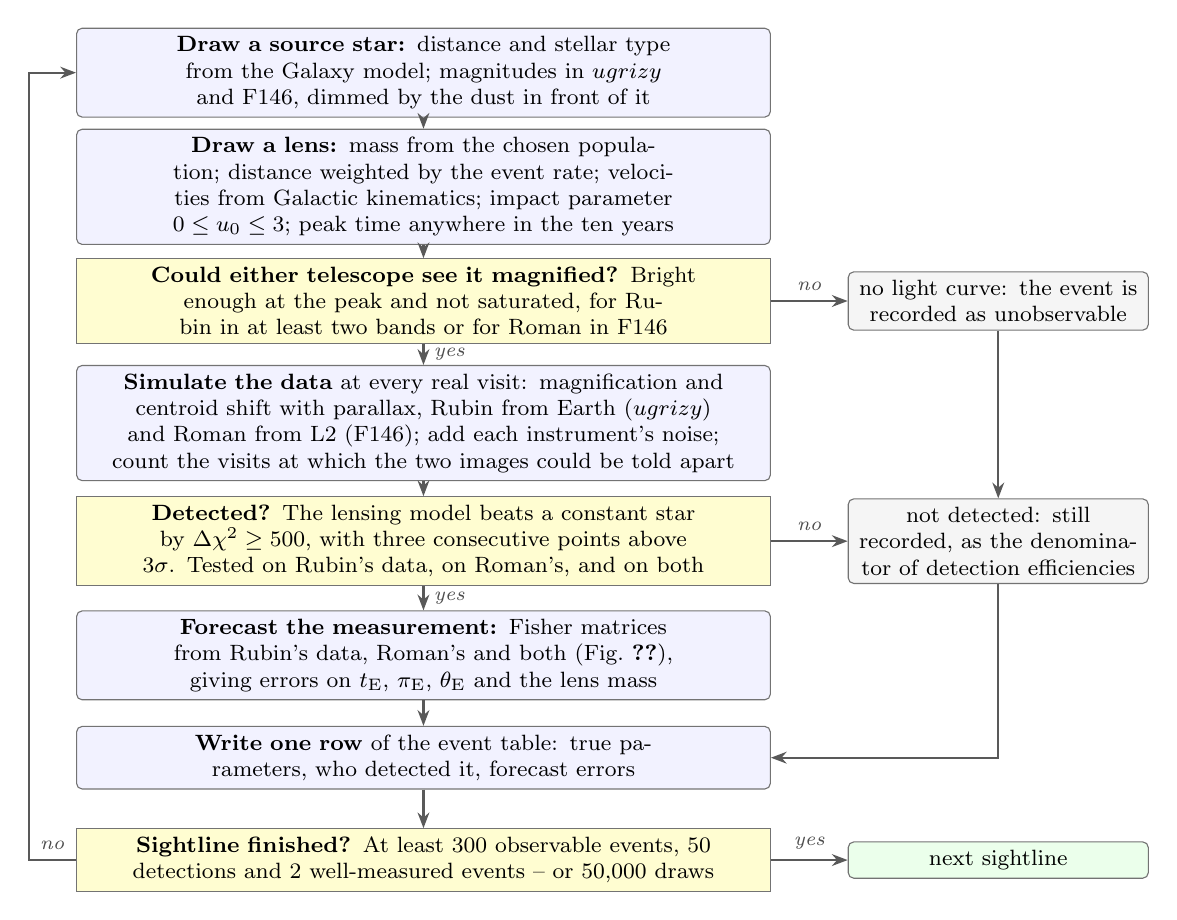
\begin{tikzpicture}
\node[box, text width=8.6cm] (src) at (0,0)
  {\textbf{Draw a source star:} distance and stellar type from the Galaxy model; magnitudes in
   $ugrizy$ and F146, dimmed by the dust in front of it};
\node[box, text width=8.6cm] (len) at (0,-1.45)
  {\textbf{Draw a lens:} mass from the chosen population; distance weighted by the event rate;
   velocities from Galactic kinematics; impact parameter ${0\le u_0\le3}$; peak time anywhere in the
   ten years};
\node[ask, text width=8.6cm] (see) at (0,-2.9)
  {\textbf{Could either telescope see it magnified?} Bright enough at the peak and not saturated,
   for Rubin in at least two bands or for Roman in F146};
\node[box, text width=8.6cm] (lc) at (0,-4.45)
  {\textbf{Simulate the data} at every real visit: magnification and centroid shift with
   parallax, Rubin from Earth ($ugrizy$) and Roman from L2 (F146); add each instrument's noise;
   count the visits at which the two images could be told apart};
\node[ask, text width=8.6cm] (det) at (0,-5.95)
  {\textbf{Detected?} The lensing model beats a constant star by ${\Delta\chi^2\ge500}$, with three
   consecutive points above $3\sigma$. Tested on Rubin's data, on Roman's, and on both};
\node[box, text width=8.6cm] (fish) at (0,-7.4)
  {\textbf{Forecast the measurement:} Fisher matrices from Rubin's data, Roman's and both
   (Fig.~\ref{fig:fisher}), giving errors on $\tE$, $\piE$, $\tetE$ and the lens mass};
\node[box, text width=8.6cm] (row) at (0,-8.7)
  {\textbf{Write one row} of the event table: true parameters, who detected it, forecast errors};
\node[ask, text width=8.6cm] (done) at (0,-10.0)
  {\textbf{Sightline finished?} At least $300$ observable events, $50$ detections and $2$
   well-measured events -- or $50{,}000$ draws};
\node[side] (no1) at (7.3,-2.9) {no light curve: the event is recorded as unobservable};
\node[side] (no2) at (7.3,-5.95) {not detected: still recorded, as the denominator of detection
  efficiencies};
\node[side, fill=green!8] (next) at (7.3,-10.0) {next sightline};
\draw[arr] (src) -- (len);
\draw[arr] (len) -- (see);
\draw[arr] (see) -- node[lab, right] {yes} (lc);
\draw[arr] (lc) -- (det);
\draw[arr] (det) -- node[lab, right] {yes} (fish);
\draw[arr] (fish) -- (row);
\draw[arr] (row) -- (done);
\draw[arr] (see) -- node[lab, above] {no} (no1);
\draw[arr] (det) -- node[lab, above] {no} (no2);
\draw[arr] (no1) -- (no2);
\draw[arr] (no2.south) |- (row.east);
\draw[arr] (done) -- node[lab, above] {yes} (next);
\draw[arr] (done.west) -- node[lab, above] {no} ++(-0.6,0) coordinate (c1)
      -- (c1 |- src.west) -- (src.west);
\end{tikzpicture}
\caption{The Monte Carlo on one sightline. Every draw is written to the event table, detected or not,
so that detection efficiencies and event rates can be computed afterwards. Only detected events are
passed to the Fisher forecast.}
\label{fig:event}
\end{figure}

\paragraph{Detection.} An event is detected when a lensing model fits the simulated data better than
a constant star by $\Delta\chi^2\ge500$, the criterion of \citet{Penny2019}'s Roman forecast. It must
also show three consecutive points more than $3\sigma$ above the baseline and have more than ten
usable points. The test is made three times, on Rubin's data alone, Roman's alone and both together,
with the same threshold. Because the $\chi^2$ of the combined data is the sum of the two surveys',
an event that either survey detects is always detected by the combination (the event table enforces
this; in one of the $85{,}061$ ordinary-lens detections the combined test failed where a
single-survey test passed, a numerical exception still under investigation). Each event is therefore
labelled \emph{detected by Rubin alone}, \emph{by Roman alone}, \emph{by both}, or \emph{only
jointly}.

\subsection{Forecasting the measurement: three Fisher matrices}
\label{sec:fisherexp}
Fitting every one of millions of simulated light curves would be prohibitively slow. Instead, for each
detected event the code computes the \emph{Fisher information matrix}: the curvature of the $\chi^2$
surface at the true parameters, built from the derivatives of the model with respect to each parameter
at every data point, weighted by that point's error,
\begin{equation}
F_{jk} = \sum_{i} \frac{1}{\sigma_i^2}\,\frac{\partial m_i}{\partial\theta_j}\,
         \frac{\partial m_i}{\partial\theta_k}.
\end{equation}
Its inverse is the covariance matrix of the best possible fit, the Cram\'er--Rao bound, given the
actual sampling and noise of the data. Two matrices are built. The \emph{photometric} one has nine
parameters: $u_0$, $\tE$, $t_0$, $\piE$, the direction of motion $\xi$, and a source magnitude and
blend fraction for each telescope, since the two see different blends through different filters. The
\emph{astrometric} one has four: $\tetE$, the two components of the source's proper motion, and $\piE$
again. The mass error follows from $\sigma(\tetE)$ and $\sigma(\piE)$
(Fig.~\ref{fig:observables}).

\begin{figure}[h]
\centering
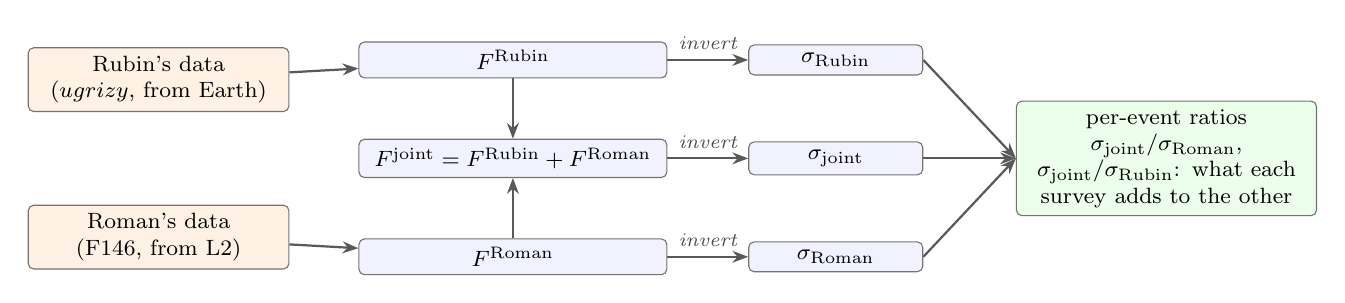
\begin{tikzpicture}
\node[box, fill=orange!10, text width=3.1cm] (rd) at (0,1.0)  {Rubin's data\\ ($ugrizy$, from Earth)};
\node[box, fill=orange!10, text width=3.1cm] (od) at (0,-1.0) {Roman's data\\ (F146, from L2)};
\node[box, text width=3.7cm] (fr) at (4.5,1.25)  {$F^{\rm Rubin}$};
\node[box, text width=3.7cm] (fo) at (4.5,-1.25) {$F^{\rm Roman}$};
\node[box, text width=3.7cm] (fj) at (4.5,0)     {${F^{\rm joint} = F^{\rm Rubin}+F^{\rm Roman}}$};
\node[box, text width=2.0cm] (sr) at (8.6,1.25)  {$\sigma_{\rm Rubin}$};
\node[box, text width=2.0cm] (sj) at (8.6,0)     {$\sigma_{\rm joint}$};
\node[box, text width=2.0cm] (so) at (8.6,-1.25) {$\sigma_{\rm Roman}$};
\node[box, fill=green!8, text width=3.6cm] (cmp) at (12.8,0)
  {per-event ratios\\ $\sigma_{\rm joint}/\sigma_{\rm Roman}$, $\sigma_{\rm joint}/\sigma_{\rm Rubin}$:
   what each survey adds to the other};
\draw[arr] (rd) -- (fr);
\draw[arr] (od) -- (fo);
\draw[arr] (fr) -- (fj);
\draw[arr] (fo) -- (fj);
\draw[arr] (fr) -- node[lab, above] {invert} (sr);
\draw[arr] (fj) -- node[lab, above] {invert} (sj);
\draw[arr] (fo) -- node[lab, above] {invert} (so);
\draw[arr] (sr.east) -- (cmp.west);
\draw[arr] (sj) -- (cmp);
\draw[arr] (so.east) -- (cmp.west);
\end{tikzpicture}
\caption{Three forecasts of the same event. The information from the two surveys adds, so
$\sigma_{\rm joint}\le\sigma_{\rm single}$ must hold for every event, which is a built-in check.
Because the three forecasts share the same source, blending, impact parameter and dust, the per-event
ratio isolates what the combination buys; a few-per-cent gain is measurable with thousands of events
rather than millions.}
\label{fig:fisher}
\end{figure}

Both matrices are built three times per event: from Rubin's data, from Roman's, and from both
(Fig.~\ref{fig:fisher}). A matrix that is singular or badly conditioned, or has fewer data points
than parameters, means the data cannot constrain the event, and it is reported as \emph{not
characterisable} rather than given an error. An event counts as \emph{characterised} when
$\tE>2\sigma_{\tE}$ and $\piE>2\sigma_{\piE}$ \citep{Abrams2025MicrolensingRubin}; for the mass we
quote the fraction measured to better than $10\%$ (or $5\%$, $1\%$).

\subsection{Covering the sky}
\label{sec:sky}
The simulation scans $67.94$\,deg$^2$ around Roman's fields with $1{,}829$ sightlines
(Fig.~\ref{fig:footsim}), far more sky than Roman's $1.47$\,deg$^2$. The reason is Rubin's field of
view. A Rubin exposure that contains part of a Roman field covers a circle $1.75^\circ$ in radius
($9.6$\,deg$^2$; \citealt{Ivezic2019LSST}),
so its far edge can lie $3.5^\circ$ beyond the Roman field. Events there are detected in the same
exposures, and a forecast that stopped at Roman's footprint would miss them. The scan is therefore
the box around Roman's fields widened by a Rubin field diameter plus a margin, and it contains
every sky position that Rubin images together with a Roman field. Of that sky ($57.5$\,deg$^2$,
from $2{,}478$ distinct Rubin pointings) $91\%$ lies inside the scan; the rest was lost to a corner
cut described below. Rubin's pointings reach $62.4$\,deg$^2$ of it ($1{,}689$ sightlines); the
other $140$ sightlines, at the edges, have no visits. Of the covered area, $59.3$\,deg$^2$ produces
detections. The remaining $77$ sightlines lie on the thinly visited rim of Rubin's coverage
($\le14$ visits each, against a median of $306$), reached the $50{,}000$-draw cap without a detection,
and carry no weight. Roman's footprint is $2.5\%$ of those $59$\,deg$^2$, but it is where the two
surveys can be compared. This is also why $64$--$73\%$ of all detections lie outside the footprint: they
are Rubin's events in the pointings around Roman's fields, and the Rubin totals for the whole scan
describe this region, not all of Rubin's bulge coverage. The sky is therefore sampled on a finer grid inside the footprint,
$0.1^\circ$ ($147$ sightlines), than outside, $0.2^\circ$ ($1{,}682$ sightlines); each sightline
carries the area it represents, which undoes the oversampling. On each sightline, draws continue
until there are enough observable events, detections and well-measured events, or until $50{,}000$
draws (Fig.~\ref{fig:event}). Inside the footprint, where Roman's $5\times10^4$ exposures detect a
large fraction of all draws, the first of these targets is the one that binds; outside, the number of
detections does.

% GENERATED by Report/overview/make_footprints.py (run from the repo root), which rebuilds the
% simulator's tiling from Bulge.h and refuses to draw unless it matches the 1,829 sightlines in
% runs/prod_bulge_20260924/run.log.
\begin{figure}[h]
\centering
\includegraphics[width=0.92\textwidth]{../../figures/footprint_20260929/footprint_simulated}
\caption{The sky the production runs scanned. Each $0.1^\circ$ cell is drawn centred on the grid
point that represents it and coloured by the number of Rubin visits at the sightline standing for
it; outside Roman's footprint one sightline represents each $0.2^\circ$ block. Grey: no survey
coverage. Dots: the sightlines. The upper-right corner ($l<-0.94^\circ$, $b>0.31^\circ$) is cut from
the scan (see text). \emph{Modelled GBTDS fields} (dashed) are the code's definition of Roman's
coverage, six circles of one WFI field's area; \emph{Roman, as simulated} (orange) are the $147$
grid sightlines that fall inside them, the cells the Monte Carlo actually samples.}
\label{fig:footsim}
\end{figure}

\begin{figure}[h]
\centering
\includegraphics[width=0.92\textwidth]{../../figures/footprint_20260929/footprint_vs_gbtds}
\caption{Roman's footprint as simulated (orange cells, dashed field circles with their centres)
over the real GBTDS detector layout (green), for the spring and autumn seasons together, since
Roman's roll angle differs between them. The background is a view from Aladin, the Strasbourg
astronomical data centre's interactive sky atlas \citep{Bonnarel2000Aladin}: optical Digitized Sky
Survey images, in which the dust lanes near the plane show as dark sky, with the Roman detector
outlines and a Galactic grid drawn over them. The image is placed in Galactic
coordinates from its own grid lines, to one pixel ($0.003^\circ$); the per-season tile area this
gives, $1.71$\,deg$^2$, matches the design's $1.7$\,deg$^2$. The real five-field block is
centred near $(l,b)=(0.49^\circ,-1.40^\circ)$ and the Galactic-centre field near
$(0.06^\circ,-0.22^\circ)$; the modelled fields sit at $b=-1.2^\circ$ and $(0^\circ,-0.125^\circ)$,
about $0.2^\circ$ and $0.1^\circ$ closer to the Galactic plane. Of the simulated footprint's
$1.47$\,deg$^2$, $1.16$\,deg$^2$ ($79\%$) lies on real detectors. It covers $59\%$ of the
$1.97$\,deg$^2$ the real tiles span over both seasons, missing mainly the southern part of the
five-field block ($b<-1.5^\circ$).}
\label{fig:footreal}
\end{figure}

Fig.~\ref{fig:footreal} sets the simulated footprint against the real one. Most of it lies on real
detectors, but the modelled fields sit about $0.2^\circ$ closer to the Galactic plane than the
adopted layout, and the real fields cover $16\%$ more sky per season. Section~\ref{sec:footunc}
estimates what this does to the results. In the model the extra area and the lower event density
farther from the plane nearly cancel, but only because the model's dust near the plane is too thin
(Section~\ref{sec:dust}); with realistic dust the real layout gives Roman $15$--$24\%$ more events
than the simulated one.

\paragraph{The corner cut.} The scan box has one corner removed, $l<-0.94^\circ$, $b>0.31^\circ$
(Fig.~\ref{fig:footsim}, upper right). The intention was to drop the corner not needed to cover
Roman's Galactic-centre field. The code drops the opposite one: this is the corner Rubin images
together with the Galactic-centre field ($4.9$\,deg$^2$ of it, against $2.7$\,deg$^2$ for the
other upper corner), and the figure shows what the code did (its sightlines match the production
runs exactly). The cost is confined to Rubin-only events outside Roman's footprint. By the event
density of simulated sightlines with the same number of Rubin visits, the corner would have added
about $1\%$ (ordinary lenses), $2.4\%$ (black holes) and $1.2\%$ (neutron stars) to the whole-scan
Rubin yields; no result inside the footprint is affected.

\subsection{From simulated events to the sky}
\label{sec:weighting}
The simulated sample is not a sample of the sky's events. The lens distance is drawn in proportion
to the event rate, but the mass is drawn from the number of lenses and the velocities from their
distributions, so the rate's factor $\sqrt{\Ml}\,v_t$ is missing: the sample over-represents long,
slow, massive events. Every pooled statistic therefore weights each event by
\begin{equation}
W = \frac{w_{\rm area}\,N_\star}{n_{\rm sim}}\;\sqrt{\Ml}\;v_t\;Z(D_s),
\end{equation}
with $w_{\rm area}$ the sightline's sky area, $N_\star$ its source-star density, $n_{\rm sim}$ its
number of draws and $Z$ the normalisation of the lens-distance distribution. The weight is validated
externally, against a published quantity from which the survey's own detection efficiency has been
removed: the efficiency-corrected mean Einstein timescale. Over all $12.2$ million draws of the
ordinary-lens run, detected or not, the weight brings the model's mean from $54.4\pm0.1$\,d
(unweighted) to $24.02\pm0.04$\,d, and to $23.5\pm0.1$\,d over $-6^\circ\le b\le-1^\circ$,
$|l|<2^\circ$. In that same region OGLE-IV measures $22.7\pm0.9$ to $25.5\pm1.2$\,d in its four
$1^\circ$ longitude bins, an inverse-variance mean of $23.8\pm0.5$\,d (\citealt{Mroz2019}, values
read from their Fig.~13). The model's errors are Monte Carlo only. Weighting costs statistical precision, so every
weighted number is quoted with the effective sample size $\Neff = (\sum W)^2/\sum W^2$
\citep{Kish1965}: the $12{,}461$ footprint detections of the ordinary-lens run weigh as
$\Neff=3{,}969$.

\paragraph{Absolute yields.} Normalising the same weights gives the expected number of events over
the ten years. For black holes and neutron stars one more quantity is needed, their abundance. Every
lens in a run is drawn from the population under test, as if the Galaxy's entire stellar mass were
black holes, say. So the result is a yield per unit abundance, $N_1$, and the expected number is
$N(F)=F\,N_1$ for a mass fraction $F$. Counts are per resolved source star: a blend of several stars
counts as one monitored object, the second detectability criterion of \citet{SajadianMakler2026},
which the published code of \citet{SajadianSahu2023} also applies. The normalisation is checked by
rebuilding the microlensing optical depth from the event-rate constants and comparing it with the
simulator's independent integral over the density; they agree to $0.1\%$ in all three populations.

% =================================================================================================
\section{The analyses, and what each tells us}
\label{sec:analyses}

Every analysis reads the event table and follows three rules. \emph{Survey comparisons are made event
by event}, as ratios of the forecasts from the same simulated data, and only then pooled. \emph{Pooled
numbers are event-rate weighted} and carry their $\Neff$; a raw count of simulated events is a Monte
Carlo sample size, never a yield. \emph{Populations are never pooled} in one weighted statistic,
because the weight contains $\sqrt{\Ml}$ of the population that was sampled. Fig.~\ref{fig:analysis}
shows the chain and Table~\ref{tab:analyses} lists the analyses.

\begin{figure}[h]
\centering
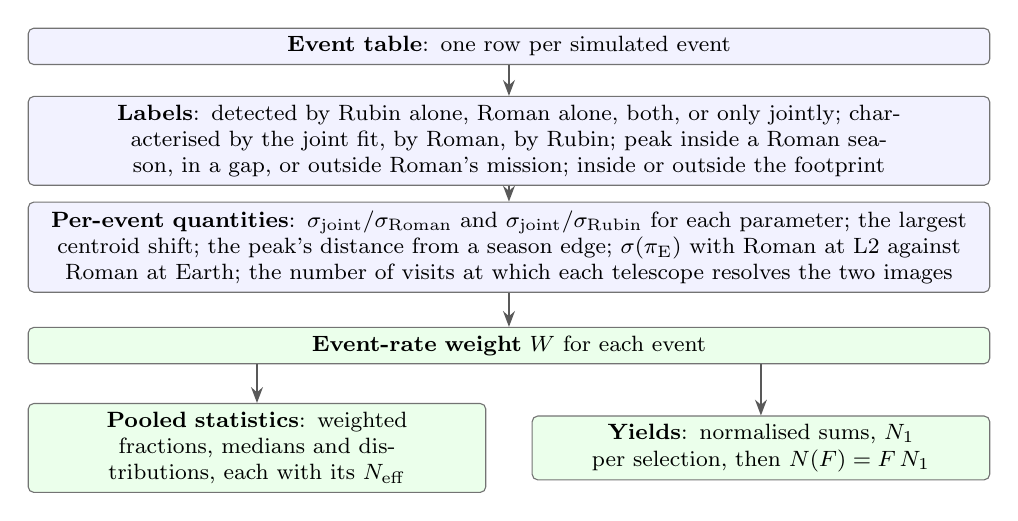
\begin{tikzpicture}
\node[box, text width=12cm] (t) at (0,0)
  {\textbf{Event table}: one row per simulated event};
\node[box, text width=12cm] (l) at (0,-1.2)
  {\textbf{Labels}: detected by Rubin alone, Roman alone, both, or only jointly; characterised by
   the joint fit, by Roman, by Rubin; peak inside a Roman season, in a gap, or outside Roman's
   mission; inside or outside the footprint};
\node[box, text width=12cm] (q) at (0,-2.55)
  {\textbf{Per-event quantities}: $\sigma_{\rm joint}/\sigma_{\rm Roman}$ and
   $\sigma_{\rm joint}/\sigma_{\rm Rubin}$ for each parameter; the largest centroid shift; the peak's
   distance from a season edge; $\sigma(\piE)$ with Roman at L2 against Roman at Earth; the number
   of visits at which each telescope resolves the two images};
\node[box, fill=green!8, text width=12cm] (w) at (0,-3.8)
  {\textbf{Event-rate weight} $W$ for each event};
\node[box, fill=green!8, text width=5.6cm] (p) at (-3.2,-5.1)
  {\textbf{Pooled statistics}: weighted fractions, medians and distributions, each with its $\Neff$};
\node[box, fill=green!8, text width=5.6cm] (y) at (3.2,-5.1)
  {\textbf{Yields}: normalised sums, $N_1$ per selection, then ${N(F)=F\,N_1}$};
\draw[arr] (t) -- (l);
\draw[arr] (l) -- (q);
\draw[arr] (q) -- (w);
\draw[arr] (w.south -| p.north) -- (p.north);
\draw[arr] (w.south -| y.north) -- (y.north);
\end{tikzpicture}
\caption{How the event table becomes results.}
\label{fig:analysis}
\end{figure}

\begin{table}[!ht]
\centering
\caption{The analyses, the question each answers, and where its result is.}
\label{tab:analyses}
\footnotesize
\begin{tabular}{p{0.16\textwidth}p{0.32\textwidth}p{0.32\textwidth}p{0.07\textwidth}}
\toprule
analysis & question & measured quantity & result \\
\midrule
who detects what & Which survey finds which events, and where? & weighted shares detected by Rubin
  alone, Roman alone, both & \S\ref{sec:who} \\
gap filling & What does Rubin recover when an event peaks while Roman is not observing? &
  $\sigma_{\rm joint}/\sigma_{\rm Roman}$ against the peak's distance from a season edge, per $\tE$
  & \S\ref{sec:gap} \\
Roman for Rubin & How much better are the events Rubin detects in the footprint measured once
  Roman's data are added? & characterised and $10\%$ fractions, Rubin alone against joint, and
  their yields; $\sigma_{\rm joint}/\sigma_{\rm Rubin}$ & \S\ref{sec:romanrubin} \\
synergy map & Which events can only the combination characterise? & characterised fraction, joint
  over single survey, across the $(\tE,\piE)$ plane & \S\ref{sec:synergy} \\
absolute precision & How well are $\tE$, $\piE$, $\tetE$ and the mass measured? & weighted
  distributions of $\sigma/{\rm value}$, per survey & \S\ref{sec:precision} \\
astrometry & Is the centroid shift measurable, and by whom? & largest shift against per-exposure and
  stacked precision; $\sigma(\tetE)$ & \S\ref{sec:astrometry} \\
satellite parallax & What does observing from L2 add? & each event forecast twice, Roman at L2 and
  at Earth & \S\ref{sec:satpar} \\
two baselines & How do the temporal and spatial parallax gains compare? & both on one scale, per
  $\tE$ bin & \S\ref{sec:two} \\
compact objects & The same questions for black-hole and neutron-star lenses & as above, per
  population & \S\ref{sec:compact} \\
resolving the images & Can either telescope see the two lensed images separately, and for which
  lenses? & visits with both images detectable and farther apart than $\mathcal{D}\sigma_a$ or the
  PSF width; resolvable if $\ge3$ \citep{SajadianMakler2026} & \S\ref{sec:resolve} \\
absolute yields & How many events and masses, for a given abundance? & $N_1$ per selection;
  $N(F)$ & \S\ref{sec:yield} \\
sample events & What do individual events look like? & full light curves and centroid tracks &
  \S\ref{sec:samples} \\
validation & Does the model reproduce known numbers? & optical depth, OGLE-IV, Penny et al.,
  Sajadian \& Sahu & \S\ref{sec:certainty} \\
\bottomrule
\end{tabular}
\end{table}

% =================================================================================================
\section{Results}
\label{sec:results}

\subsection{The simulated sample}
Three runs were made, identical except for the lens population, over the same sightlines
(Table~\ref{tab:runs}). The counts in the table are Monte Carlo sample sizes: they set the statistical
precision of the results, not the number of events the surveys will see, which is in
Section~\ref{sec:yield}. Sections~\ref{sec:who}--\ref{sec:two} use the ordinary-lens run; the
comparison of what each survey adds to the other (Section~\ref{sec:romanrubin}) and the resolution
of the two images (Section~\ref{sec:resolve}) cover all three. Every error bar is the $1\sigma$
Monte Carlo uncertainty: a bootstrap over simulated events for fractions and medians, and Poisson
on the draws for yields. Modelling uncertainties are discussed separately in
Section~\ref{sec:certainty} and are larger.

\textbf{The numbers in this section are as simulated.} The simulation's dust is too thin near the
Galactic plane, which inflates the absolute yields; Section~\ref{sec:dust} corrects for it, and the
abstract, the summary and Table~\ref{tab:corrected} quote the corrected values with their
uncertainties. The corrections lower Roman's yields by a third and Rubin's by more than half, but
leave the per-event results of Table~\ref{tab:corrected} essentially as they are. The gap-filling
gains of Section~\ref{sec:gap} were not corrected: the extra dust dims Rubin's sources $4.3$ times as
much as Roman's, so they are upper limits.

% Source: runs/prod_*_20260924/run.log and the y1 logs (figures/yield_20260925/<pop>/y1.log).
\begin{table}[h]
\centering
\caption{The three production runs. Detections are simulated events (Monte Carlo sample sizes), not
yields.}
\label{tab:runs}
\small
\begin{tabular}{lrrr}
\toprule
 & ordinary lenses & black holes & neutron stars \\
\midrule
mass function & Kroupa + remnants & log-uniform, $3$--$1000\,\Msun$ & $1.35\pm0.15\,\Msun$ \\
simulated events & $12.2$ million & $6.5$ million & $8.4$ million \\
simulated detections, any survey & $85{,}061$ & $101{,}515$ & $93{,}185$ \\
\quad of which inside Roman's footprint & $12{,}461$ & $24{,}186$ & $19{,}058$ \\
\bottomrule
\end{tabular}
\end{table}

\subsection{Who detects what, and why}
\label{sec:who}
% Source: figures/u1_20260929/u1_numbers.md (shares, yields, dust, peak coverage).
Weighted by the event rate, $(66.8\pm0.5)\%$ of ordinary-lens detections are made by Rubin alone,
$(29.2\pm0.4)\%$ by Roman alone and $(3.8\pm0.2)\%$ by both ($\Neff=9{,}465$); for black holes and
neutron stars the shares are similar (Table~\ref{tab:compact}). The large Rubin share is sky area:
Rubin covers the $59$\,deg$^2$, Roman $1.47$\,deg$^2$ of it, and $(63.8\pm0.5)\%$ of all detections
fall outside Roman's footprint. Inside the footprint the balance reverses. There Roman detects
$(8.19\pm0.14)\times10^4$ events over the decade and Rubin $(1.68\pm0.06)\times10^4$, and Roman also
detects $(56\pm2)\%$ of the events Rubin detects there; the rest peak while Roman is not observing.
Two physical causes compound. The first is dust: at the model's median extinction of footprint
detections, $A_r=3.04\pm0.05$\,mag ($A_V\approx3.6$), it dims Rubin's $r$-band source by $3.0$\,mag
and Roman's F146 source by $0.7$\,mag. The model's dust near the plane is too thin
(Section~\ref{sec:dust}), so the real contrast is larger. The second is sampling: Roman has $\sim\!20$ times as many data points
on each sightline. The simplest summary came out of the sample events (Section~\ref{sec:samples}):
\emph{when Roman observes the peak, Roman detects the event.} Among the $917$ simulated footprint
events that Rubin detects and Roman does not, only $1$ peaks inside a Roman season ($116$ peak in a
gap, $800$ outside Roman's mission). And only $(4.4\pm0.4)\%$ of Roman's ordinary-lens detections
($2.9$--$3.9\%$ for compact objects) have no Roman exposure within $\pm2\tE$ of the peak, so Roman's
yield is of events it saw while they were magnified.

\subsection{Gap filling: what Rubin recovers from Roman's season gaps}
\label{sec:gap}

\begin{figure}[h]
\centering
\includegraphics[width=\textwidth]{f2_gap_filling}
\caption{What Rubin adds as an event's peak moves out of a Roman season into a gap. Left: median
per-event $\sigma_{\rm joint}(\tE)/\sigma_{\rm Roman}(\tE)$ against distance to the nearest season
edge, per $\tE$ bin (solid: weighted; dashed: raw), over the $9{,}764$ footprint detections peaking
within Roman's mission ($\Neff=3{,}471$; the stamp's $9{,}465$ is that of all detections). Right:
fraction of events the joint fit characterises and Roman alone does not. Shaded: inside a season.}
\label{fig:f2}
\end{figure}

% Source: figures/wp_20260926/f2_tE.log, f2_piE.log; errors and the three coverage columns from
% figures/u1_20260929/u1_numbers.md ("gap filling: Roman's coverage of the same events").
\begin{table}[h]
\centering
\caption{Median $\sigma_{\rm joint}/\sigma_{\rm Roman}$ for $10$--$30$\,d footprint events, by where
the peak falls, with bootstrap errors (below $10^{-4}$ for the control row). A peak ``in a gap'' does
not mean Roman has no data on the event: every event here lies on a sightline Roman observes
throughout its mission (at least $46{,}112$ recorded exposures each) and has a Roman forecast. The
last three columns say what Roman saw of it, as weighted percentages of the row: the share Roman
detects, the share Rubin detects, and the share with no Roman exposure within $\pm2\tE$ of the peak.
Events: simulated events in the row. Each row below the first is a subset of the one above it.}
\label{tab:gap}
\small
\setlength{\tabcolsep}{3.5pt}
\begin{tabular}{lcccccrr}
\toprule
 & \multicolumn{2}{c}{$\sigma_{\rm joint}/\sigma_{\rm Roman}$} & Roman & Rubin & no Roman & & \\
peak position & $\tE$ & $\piE$ & detects & detects & point near peak & events & $\Neff$ \\
\midrule
anywhere in a gap              & $0.973\pm0.010$ & $0.984\pm0.006$ & $95.5\pm0.7$ & $16.7\pm1.3$ & $11.6\pm1.2$ & $1{,}359$ & $670$ \\
$>15$\,d past a season edge    & $0.83\pm0.07$ & $0.89\pm0.04$ & $91.8\pm1.3$ & $20.7\pm1.9$ & $21.3\pm2.1$ & $778$ & $376$ \\
$>30$\,d past                  & $0.44\pm0.15$ & $0.70\pm0.09$ & $82.5\pm2.7$ & $27.4\pm3.3$ & $41.9\pm3.9$ & $365$ & $177$ \\
$>45$\,d past                  & $\mathbf{0.08\pm0.06}$ & $\mathbf{0.18\pm0.07}$ & $66.5\pm6.1$ & $44.7\pm6.2$ & $72.8\pm5.5$ & $122$ & $62$ \\
\midrule
in a season (control)          & $1.0000$ & $1.0000$ & $99.93\pm0.06$ & $9.0\pm0.8$ & $0$ & $1{,}835$ & $888$ \\
\bottomrule
\end{tabular}
\end{table}

For $10$--$30$\,d events pooled over the gaps, Rubin improves Roman's $\tE$ precision by only
$(2.7\pm1.0)\%$. With Roman's sources as bright as they are in F146, Roman's coverage of the wings
settles any event that peaks near a season edge: Roman itself detects $(95.5\pm0.7)\%$ of these
in-gap events, most of them from the wings, and only $(11.6\pm1.2)\%$ have no Roman exposure within
$\pm2\tE$ of the peak. The gain is large, sharp and physical only where
the \emph{whole event} falls inside a gap: for a $10$--$30$\,d event peaking more than $45$ days from
either edge, the joint forecast is essentially Rubin's, and it is better than Roman's alone by an
order of magnitude (median ratio $0.08\pm0.06$, i.e.\ a factor $\gtrsim7$). For events of $30$\,d
and longer the pooled in-gap medians are $0.999$--$1.000$. Gap filling also adds events:
$(2.0\pm0.4)\%$ of in-gap footprint detections are characterised jointly and not by Roman alone,
rising to $(7\pm3)\%$ ($10$--$30$\,d) and $(10\pm3)\%$ ($30$--$100$\,d) beyond $45$\,d. The deepest
row of Table~\ref{tab:gap} rests on $\Neff=62$, which is why its errors are large. It also shows the
limit of the wing detections noted in Section~\ref{sec:next}: $(72.8\pm5.5)\%$ of those events have no
Roman exposure near the peak, yet $(66.5\pm6.1)\%$ still pass Roman's detection test, on a slow, faint
brightening summed over tens of thousands of exposures. All of these gains are as simulated. The
dust correction of Section~\ref{sec:dust} cannot be applied to them, because for medians of per-event
ratios it re-weights events only by whether they are still detected, not by how their precision
changes; the extra dust dims Rubin's
sources $4.3$ times as much as Roman's, so Rubin's share of the joint forecast, and with it every gain
in this section, can only shrink. Only a run with the corrected dust will say by how much.

\subsection{What Roman adds to Rubin}
\label{sec:romanrubin}

The question can be turned round: for the events \emph{Rubin} detects, what does adding Roman's data
buy? Only events inside the footprint can gain, and they are a minority of Rubin's detections --
$(9.6\pm0.4)\%$ for ordinary lenses, $(7.4\pm0.2)\%$ for black holes and $(8.2\pm0.2)\%$ for
neutron stars -- because Rubin's other $\sim\!90\%$ lie where Roman does not look. For those events,
however, the gain is not a refinement but a change of kind (Table~\ref{tab:romanrubin}).

% Source: figures/u1_20260929/u1_numbers.md, sections "what Roman adds, over Rubin's footprint
% detections" and "what Rubin adds, over Roman's footprint detections".
\begin{table}[h]
\centering
\caption{What Roman adds to the events Rubin detects inside the footprint, per population. Each
cell is Rubin alone $\to$ joint, as a weighted percentage of Rubin's footprint detections;
\emph{characterised} means $\tE>2\sigma_{\tE}$ and $\piE>2\sigma_{\piE}$. The medians are of the
per-event ratio $\sigma_{\rm joint}/\sigma_{\rm Rubin}$. Yields are per unit abundance $N_1$ (ordinary
lenses: $F=1$), footprint, ten years. The last row gives the reverse, what Rubin adds to Roman's own
footprint detections, for scale.}
\label{tab:romanrubin}
\footnotesize
\setlength{\tabcolsep}{3pt}
\begin{tabular}{lccc}
\toprule
 & ordinary lenses & black holes & neutron stars \\
\midrule
Rubin's footprint detections, $N_1$ & $16{,}830\pm640$ & $1{,}811\pm40$ & $11{,}560\pm280$ \\
\quad Roman also detects [\%] & $56\pm2$ & $96.4\pm0.3$ & $65\pm1$ \\
characterised [\%] & $5.0\pm1.4\to26.0\pm1.7$ & $13.4\pm0.7\to78.9\pm0.9$ & $4.9\pm0.3\to37.3\pm1.1$ \\
$\tE$ to $10\%$ [\%] & $4.4\pm1.4\to33.3\pm1.8$ & $17.6\pm0.9\to75.2\pm1.0$ & $5.8\pm0.5\to42.4\pm1.2$ \\
$\piE$ to $10\%$ [\%] & $0.8\pm0.1\to12.4\pm1.5$ & $2.2\pm0.3\to49.9\pm1.2$ & $0.9\pm0.1\to16.7\pm0.7$ \\
$\tetE$ to $10\%$ [\%] & $0.04\pm0.02\to60.7\pm1.8$ & $41.5\pm1.2\to98.8\pm0.2$ & $0.4\pm0.1\to77.7\pm1.0$ \\
$\Ml$ to $10\%$ [\%] & $0.007\pm0.005\to8.9\pm1.4$ & $0.45\pm0.13\to49.5\pm1.2$ & $0.001\pm0.001\to14.9\pm0.7$ \\
\midrule
median $\sigma_{\rm joint}/\sigma_{\rm Rubin}$, $\tE$ & $0.16\pm0.02$ & $0.065\pm0.003$ & $0.13\pm0.01$ \\
\qquad\qquad\quad $\piE$ & $0.13\pm0.01$ & $0.039\pm0.001$ & $0.105\pm0.006$ \\
\qquad\qquad\quad $\Ml$ & $0.10\pm0.01$ & $0.036\pm0.001$ & $0.081\pm0.006$ \\
\midrule
characterised, $N_1$ & $840\pm230\to4{,}380\pm330$ & $242\pm13\to1{,}429\pm36$ & $571\pm37\to4{,}310\pm150$ \\
$\Ml$ to $10\%$, $N_1$ & $1.1\pm0.8\to1{,}490\pm260$ & $8\pm2\to896\pm28$ & $0.15\pm0.10\to1{,}726\pm80$ \\
\midrule
reverse, Rubin for Roman: $\Ml$ to $10\%$ [\%] & $2.36\pm0.32\to2.59\pm0.33$ & $12.7\pm0.4\to14.5\pm0.4$ & $3.9\pm0.2\to4.5\pm0.2$ \\
\bottomrule
\end{tabular}
\end{table}

Rubin alone characterises one in eight of its black-hole detections in the footprint and one in
twenty of the others; with Roman's data added, $26$--$79\%$ are characterised, a factor
$5.2\pm1.3$ (ordinary lenses), $5.9\pm0.3$ (black holes) and $7.6\pm0.5$ (neutron stars) more.
The median event's timescale becomes $6$--$15$ times more precise and its parallax $8$--$26$ times.
The largest change is in the mass. Rubin by itself measures essentially no lens masses. For ordinary
lenses and neutron stars its seeing-limited astrometry cannot reach $\tetE$; for black holes it does
reach $\tetE$ in $42\%$ of events, but its parallax is measured to $10\%$ in only $2\%$. With Roman's
photometry and astrometry added, a tenth of Rubin's ordinary-lens detections, a seventh of its
neutron-star detections and half of its black-hole detections have masses to $10\%$. The reverse gain, what Rubin adds to Roman's own
detections, is $10$--$14\%$ in the same quantity (last row). The asymmetry has the same cause as the
detection results. Toward the bulge Rubin's optical photometry is sparse and heavily extincted, so on
the same event Roman holds most of the information, and adding Roman to Rubin changes the answer
while adding Rubin to Roman only refines it.

For most of these events Roman is not only adding information but has detected the event itself:
it also detects $56\%$ of Rubin's ordinary-lens footprint detections, $65\%$ of the neutron-star and
$96\%$ of the black-hole ones. The rest peak while Roman is not observing, and Roman still
contributes the wings.
Seen from Rubin's side, the result is this: of Rubin's $1.75\times10^5$ ordinary-lens detections over
the decade, the $1.7\times10^4$ that fall in Roman's footprint are the ones that can be turned into
measurements of $\tE$, $\piE$ and the lens mass.

\subsection{What the combination characterises that neither survey does}
\label{sec:synergy}

\begin{figure}[h]
\centering
\includegraphics[width=\textwidth]{f3_characterization_map}
\caption{Characterised fraction, joint over single survey, in the $(\tE,\piE)$ plane, weighted.
(a) what Rubin adds to Roman; (b) what Roman adds to Rubin (hatched: Rubin alone characterises
nothing and the joint fit does). Dashed: constant lens mass at the median $\mu_{\rm rel}$.}
\label{fig:f3}
\end{figure}

Figure \ref{fig:f3} shows how much each survey helps the other. Panel (a) is pale everywhere: inside the footprint, adding Rubin barely changes which events are
characterised. Panel (b) is the reverse. Roman multiplies what Rubin can characterise, most of all for
short events: at $3$--$10$\,d Rubin alone characterises none and the joint fit does, and at
$10$--$30$\,d with small parallax ($\piE\sim0.03$--$0.1$) the joint fit characterises $66$ times as
many. Panel (b) is over all detections, most of them outside the footprint where Roman has no data,
so it shows where in the $(\tE,\piE)$ plane Roman helps rather than by how much;
Section~\ref{sec:romanrubin} gives the size of the gain on the events Roman can reach. Of the $12{,}461$ simulated footprint detections (raw counts), the joint fit
characterises $3{,}948$, Roman alone $3{,}412$ and Rubin alone $670$; $358$ are characterised jointly
and by neither survey alone, events in which each survey holds part of the information and only
their sum constrains both $\tE$ and $\piE$.

\subsection{Absolute precision}
\label{sec:precision}

\begin{figure}[h]
\centering
\includegraphics[width=\textwidth]{f4_fisher_precision}
\caption{Fractional $1\sigma$ forecasts per survey over the $12{,}461$ footprint detections
($\Neff=3{,}969$): (a)--(c) fitted parameters, (d) lens mass, (e) the invariant
$\sigma_{\rm joint}\le\sigma_{\rm single}$ event by event, (f) condition numbers. Curves are
normalised to the full sample, so an unmeasured event lowers a curve.}
\label{fig:f4}
\end{figure}

% Source: figures/wp_20260926/f4.log; errors from figures/u1_20260929/u1_numbers.md.
\begin{table}[h]
\centering
\caption{Weighted percentage of the $12{,}461$ footprint detections ($\Neff=3{,}969$) measured to
better than $10\%$, ordinary lenses.}
\label{tab:f4}
\begin{tabular}{lccc}
\toprule
 & joint & Roman alone & Rubin alone \\
\midrule
$\tE$      & $13.2\pm0.5$ & $11.6\pm0.5$ & $0.8\pm0.3$ \\
$\piE$     & $3.7\pm0.3$  & $3.3\pm0.3$  & $0.15\pm0.02$ \\
$\tetE$    & $50.5\pm0.8$ & $50.3\pm0.8$ & $0.13\pm0.04$ \\
$\Ml$      & $2.4\pm0.3$  & $2.2\pm0.3$  & $0.001\pm0.001$ \\
\bottomrule
\end{tabular}
\end{table}

The joint column sits within $1.6$ percentage points of Roman's, and Rubin alone measures almost
nothing to $10\%$ inside the footprint. The parallax is the limiting measurement: $\tetE$ is measured
to $10\%$ for half of all events, $\piE$ for $4\%$, and the mass, which needs both, for $2.4\%$.
Unweighted, the fractions are larger ($\Ml$: $9.9\%$ joint), because the raw sample over-represents the
slow, massive events that are easiest to characterise; this is why the weighting matters. Panel (e)
holds except for round-off ($\le1.0007$) and one lens-mass forecast on a nearly singular matrix
(condition number $>10^9$).

\subsection{The astrometric shift, and who measures the Einstein radius}
\label{sec:astrometry}

\begin{figure}[h]
\centering
\includegraphics[width=\textwidth]{h5_astrometric_shift}
\caption{The astrometric signal, footprint detections ($\Neff=3{,}969$): (a) maximum centroid
shift against per-exposure precision; (b) signal relative to one exposure and to the stack;
(c) where the astrometric maximum falls relative to Roman's seasons; (d) forecast
$\sigma(\tetE)/\tetE$; (e) the joint-versus-single invariant; (f) the $(\piE,\tetE)$ plane.}
\label{fig:h5}
\end{figure}

\begin{figure}[h]
\centering
\includegraphics[width=\textwidth]{h5_astrometry_summary}
\caption{The four claims the astrometric result rests on, each with its check: (a) signal against
one exposure and the stack; (b) which instrument measures $\tetE$; (c) the lens mass; (d) precision
improving with the deflection.}
\label{fig:h5sum}
\end{figure}

% Source: figures/wp_20260926/h5.log, h5sum.log.
The median maximum shift of an ordinary event is $0.124\pm0.002$\,mas, against Roman's median
per-exposure precision of $2.75\pm0.09$\,mas for these sources; only $(0.22\pm0.07)\%$ of events
exceed one exposure. \textbf{The
measurement exists entirely through averaging}: over $\sim\!5\times10^4$ exposures an independent
error falls to $0.012$\,mas, and the median signal stands at $10\sigma$. That factor $\sim\!224$ is
the whole astrometric result, and it rests on an assumption discussed in Section~\ref{sec:certainty}.
Given it, $\tetE$ is Roman's measurement: the median $\sigma(\tetE)/\tetE$ is $0.098\pm0.003$ joint,
$0.099\pm0.003$ Roman alone and $2.30\pm0.06$ Rubin alone, since Rubin's seeing-limited images are ten
times wider.
\textbf{The lens mass still benefits from both surveys}: $143$ simulated footprint events have a
$10\%$ mass from the joint fit and from neither survey alone ($319$ at $30\%$). In yield terms the
combination raises the number of $10\%$ masses over the decade from $1{,}930\pm260$ to
$2{,}120\pm270$ (Table~\ref{tab:n1}); the two share most of their events, so the gain itself is
measured more precisely, a factor $1.10\pm0.03$. The astrometric maximum falls $\sim\!1.4\,\tE$ from the photometric peak, and
lies across a season edge from it for $(39.6\pm0.8)\%$ of events, so the two signals are often
caught in different seasons.

\subsection{Satellite parallax: Roman at L2 against Roman at Earth}
\label{sec:satpar}

\begin{figure}[h]
\centering
\includegraphics[width=0.9\textwidth]{h3a_where}
\caption{Per-event $\sigma_{\piE}$(Roman at L2)$/\sigma_{\piE}$(Roman at Earth) against the
observer separation in Einstein radii, coloured by $\tE$; the same event characterised twice.}
\label{fig:h3a}
\end{figure}

% Source: figures/wp_20260926/h3.log.
To isolate the satellite parallax, every detected event is forecast twice from the same simulated
data: once with Roman at L2 and once with Roman placed at Earth. Over $10{,}806$ Roman-covered events
($\Neff=3{,}521$) the median ratio of the two $\sigma(\piE)$ is $0.99110\pm0.00009$. The gain is
\textbf{under $1\%$, but real}: $(92.3\pm0.4)\%$ of events improve, and control events with no Roman
data near the peak give exactly $1.000000$. The $(1.2\pm0.1)\%$ of events that improve by more than a
factor of two are short
($\tE\approx5$\,d), fairly high-magnification events, for which the $0.01$\,AU between L2 and Earth
is the largest fraction of the Einstein radius projected onto the observer's plane
(Fig.~\ref{fig:h3a}). For black holes and neutron stars, whose projected Einstein radii are larger
and whose events are longer, the gain is nil (median exactly $1$).

\subsection{Two baselines on one scale}
\label{sec:two}

\begin{figure}[h]
\centering
\includegraphics[width=0.8\textwidth]{h3c_honest}
\caption{Median improvement in $\sigma(\piE)$ per $\tE$ bin, weighted. Blue: Roman at L2 against
Roman at Earth (spatial baseline). Orange: joint against Roman alone for footprint events peaking in
a gap (temporal baseline).}
\label{fig:h3c}
\end{figure}

A second observer helps the parallax in two ways: across space (L2 against Earth) and across time
(Rubin observing while Roman cannot). On one scale they are the same size for $10$--$30$\,d events:
$(1.6\pm0.6)\%$ (temporal, pooled over the gaps) against $(0.92\pm0.01)\%$ (spatial). Each is large only in its own corner:
the spatial baseline for short, high-magnification events, the temporal one for events that fall
entirely inside a gap.

\subsection{Black holes and neutron stars}
\label{sec:compact}

\begin{figure}[h]
\centering
\includegraphics[width=\textwidth]{p6_synergy}
\caption{Compact-object runs. (a) Weighted detection share by survey. (b) Median joint/single
$\sigma(\tE)$ against $\tE$, over events characterised by both surveys.}
\label{fig:p6}
\end{figure}

% Source: figures/prod_20260925/p6_synergy_resolution.log, p7_forecast_figures.log; errors from
% figures/u1_20260929/u1_numbers.md (which reproduces every logged value).
\begin{table}[h]
\centering
\caption{Compact-object runs. Shares, shifts and $10\%$ fractions are weighted over all detections
($\Neff=17{,}638$ black holes, $17{,}086$ neutron stars); the $10\%$ fractions are over the events
whose Roman forecast exists. The $\sigma$ ratios are weighted medians over the events whose
photometric Fisher matrices both surveys can invert ($23{,}961$ black-hole, $18{,}895$ neutron-star
events).}
\label{tab:compact}
\small
\setlength{\tabcolsep}{4pt}
\begin{tabular}{lrr}
\toprule
 & black holes & neutron stars \\
\midrule
detected by Rubin only [\%] & $72.9\pm0.3$ & $69.6\pm0.3$ \\
\quad by Roman only / by both [\%] & $21.5\pm0.3$ / $5.6\pm0.1$ & $26.3\pm0.3$ / $3.9\pm0.1$ \\
median $\sigma_{\rm joint}/\sigma_{\rm Roman}$, $\tE$ & $0.9971\pm0.0003$ & $0.9989\pm0.0001$ \\
\qquad\qquad\quad $\piE$ / $\tetE$ & $0.9978\pm0.0002$ / $0.9990\pm0.0001$ & $0.9991\pm0.0001$ / $0.9988\pm0.0001$ \\
median $\sigma_{\rm joint}/\sigma_{\rm Rubin}$, $\tE$ & $0.0216\pm0.0007$ & $0.0084\pm0.0003$ \\
\qquad\qquad\quad $\piE$ / $\tetE$ & $0.0100\pm0.0003$ / $0.0414\pm0.0009$ & $0.0075\pm0.0002$ / $0.0350\pm0.0006$ \\
median max.\ centroid shift [mas]      & $3.60\pm0.03$ & $0.264\pm0.001$ \\
fraction above Roman's $1.1$\,mas floor [\%] & $90.4\pm0.1$ & $0.58\pm0.03$ \\
Roman to $10\%$: $\tE$ / $\piE$ [\%] & $23.6\pm0.5$ / $12.9\pm0.4$ & $16.0\pm0.4$ / $4.5\pm0.2$ \\
\qquad\qquad\quad $\tetE$ / $\Ml$ [\%] & $97.0\pm0.1$ / $12.6\pm0.4$ & $67.2\pm0.5$ / $3.7\pm0.2$ \\
\bottomrule
\end{tabular}
\end{table}

Roman is the only detector of $21$--$26\%$ of compact-object events, from $2.5\%$ of the sky. On
events both surveys constrain, Rubin adds almost nothing to Roman: the median ratio is
$0.997$--$0.999$, flat over four decades of $\tE$, including multi-year events where Rubin's
decade-long baseline should matter most. The mirror image, what Roman does to Rubin's forecast of
the same events, is a median factor $46$ (black holes) and $120$ (neutron stars) in $\sigma(\tE)$
(Table~\ref{tab:compact}). Most of these events are Roman detections that Rubin only barely
constrains; Section~\ref{sec:romanrubin} gives the gain on the events Rubin itself detects.
The reason is the dust: Rubin's $r$-band source is several magnitudes fainter than Roman's F146 one.
\textbf{The expectation that long events need Rubin for the parallax is not borne out}; Roman's ten
seasons over $4.7$ years already sample enough of Earth's orbit. Black holes exceed Roman's
per-exposure astrometric floor for $90\%$ of detections, so their $\tetE$, unlike that of ordinary
lenses, does not depend on averaging exposures; $97\%$ are measured to $10\%$. The mass is then limited
by the parallax, measured to $10\%$ for $13\%$ of black-hole events: the heaviest lenses have the
smallest $\piE$. The same large $\tetE$ can make the two images separately visible, the subject of
Section~\ref{sec:resolve}.

\begin{figure}[h]
\centering
\includegraphics[width=\textwidth,trim=0 14 508 0,clip]{p7_precision}
\caption{Weighted cumulative distribution of the fractional error, per survey and population.
Each curve is over its own characterised set, so a Roman curve above the joint one is a difference
of samples, not a violation of $\sigma_{\rm joint}\le\sigma_{\rm single}$.}
\label{fig:p7}
\end{figure}

\FloatBarrier
\subsection{Resolving the two images}
\label{sec:resolve}

\paragraph{Method.} A point lens forms two images of the source, one on each side of it, separated
by $\Delta\theta=\tetE\sqrt{u^2+4}$ (Section~\ref{sec:science}). We follow
\citet{SajadianMakler2026}, who asked whether Rubin could see the two images of black-hole lenses
toward the Magellanic Clouds. At every visit it records, the simulation asks two questions.
\emph{(i) Would both images be detected on their own?} Each image's magnitude is the source's own
flux times its magnification $A_\pm$, with the light of unrelated blended stars not added back, which
makes the fainter image fainter and the test conservative; both must lie between saturation and the
single-visit depth of that filter. \emph{(ii) Are they farther apart than the telescope can
separate?} An event counts as \emph{resolvable} if at least three visits pass both tests. Because
the separation grows only as the minor image fades, the count must be made visit by visit; it cannot
be reconstructed from an event's summary parameters.

The resolution bar in (ii) is where the answer depends on assumptions. \citet{SajadianMakler2026} take
$\Delta\theta\ge\mathcal{D}\sigma_a$, with $\sigma_a$ the per-visit astrometric precision of a single
star and $\mathcal{D}$ growing with signal-to-noise and with the brightness difference of the two
images: $\mathcal{D}\approx5$ at the detection limit, $\approx20$ at a signal-to-noise of $100$ for
images of similar brightness, and larger when one image is several magnitudes fainter. We record both
anchors, $\mathcal{D}=5$ and $\mathcal{D}=20$. The criterion was built for Rubin's seeing-limited
images. On Roman's $1.1$\,mas floor, $\mathcal{D}=5$ would mean separating two point sources
$5.5$\,mas apart, a twentieth of its diffraction-limited point-spread function (FWHM $105$\,mas in
F146; \citealt{STScIWFIQuickRef}), and
whether the shape of one blended image allows that is doubtful. A third, conservative bar is
therefore recorded as well: $\Delta\theta$ at least the PSF width ($105$\,mas for Roman,
$\approx1''$ for Rubin). For Roman the truth plausibly lies between the $\mathcal{D}$ bars and the
PSF bar.

\paragraph{A correction to the depth.} The production runs took Roman's single-exposure depth in
F146 as $29$\,mag, a placeholder. Roman's own photometric error model, the one every simulated Roman
point uses, reaches $5\sigma$ at $25.5$\,mag. Since the images separate only as the minor image
fades, the depth matters here, although it barely matters for detection: only $0.3$--$1\%$ of Roman's
detections have a baseline fainter than $25.5$\,mag. The per-visit counts were therefore rebuilt for
every Roman detection on Roman's real list of $50{,}401$ exposures, with the same magnitudes, errors
and bars as the simulator but without parallax. With the depth at $29$\,mag this reproduces the
simulator's own verdict for $99.5$--$100\%$ of events individually, and its resolvable fractions to
within $0.1$ percentage points. The Roman numbers quoted below use the realistic $25.5$\,mag. Rubin's
depths were its real single-visit ones, and its numbers are the simulator's.

% Source: figures/u1_20260929/u1_numbers.md (Rubin; Roman as simulated) and
% figures/u1_20260929/u2_resolution_depth.csv (Roman at the 5-sigma depth, semi-analytic re-count).
\begin{table}[h]
\centering
\caption{Probability that the two images are resolvable ($\ge3$ qualifying visits), as a weighted
percentage of each telescope's own detections, and the yield of such events. Roman: at its $5\sigma$
single-exposure depth, F146\,$=25.5$ (in brackets: as simulated, with the $29$\,mag placeholder).
Rubin: as simulated. Yields $N_1$ are per unit abundance (ordinary lenses: $F=1$) over ten years;
Roman's are in its footprint, Rubin's over the whole scan.}
\label{tab:resolve}
\footnotesize
\setlength{\tabcolsep}{3pt}
\begin{tabular}{lccc}
\toprule
 & ordinary lenses & black holes & neutron stars \\
\midrule
Roman, $\mathcal{D}=5$ [\%]  & $1.4\pm0.4$ \;($5.1\pm0.5$) & $45.4\pm0.6$ \;($65.5\pm0.5$) & $2.9\pm0.1$ \;($14.9\pm0.4$) \\
Roman, $\mathcal{D}=20$ [\%] & $<0.001$ \;($0.6\pm0.3$) & $22.1\pm0.5$ \;($30.9\pm0.5$) & $0.022\pm0.006$ \;($0.35\pm0.05$) \\
Roman, PSF [\%]              & $0$ \;($0$) & $0.31\pm0.04$ \;($0.68\pm0.07$) & $<10^{-4}$ \;($0.001\pm0.001$) \\
Rubin, $\mathcal{D}=5$ [\%]  & $0.011\pm0.010$ & $5.5\pm0.2$ & $0.0002\pm0.0001$ \\
Rubin, $\mathcal{D}=20$ / PSF [\%] & $0$ / $0$ & $0.031\pm0.006$ / $0.0003\pm0.0002$ & $0$ / $0$ \\
\midrule
Roman $N_1$, $\mathcal{D}=5$ / $20$ / PSF & $1{,}140\pm290$ / $0.3$ / $0$ & $3{,}810\pm60$ / $1{,}860\pm50$ / $26\pm4$ & $1{,}700\pm90$ / $13\pm3$ / $0.03$ \\
Rubin $N_1$, $\mathcal{D}=5$ & $20\pm18$ & $1{,}330\pm60$ & $0.3\pm0.1$ \\
\bottomrule
\end{tabular}
\end{table}

\begin{figure}[h]
\centering
\includegraphics[width=\textwidth]{../../figures/u1_20260929/p6_resolution}
\caption{Resolving the two images, as simulated (Roman's depth at the $29$\,mag placeholder; at its
real $5\sigma$ depth Roman's probabilities fall by the factors in Table~\ref{tab:resolve}). (a) The
probability per population, telescope and bar, over each telescope's detections. (b) The same at
$\mathcal{D}=5$ against lens mass.}
\label{fig:resolve}
\end{figure}

\paragraph{Results.} The three bars differ by two orders of magnitude, and that spread, not the
Monte Carlo error, is the real uncertainty (Table~\ref{tab:resolve}, Fig.~\ref{fig:resolve}).
\emph{Black holes} are the only population for which resolution is common: Roman resolves the images
of $(45.4\pm0.6)\%$ of its black-hole detections at $\mathcal{D}=5$, $(22.1\pm0.5)\%$ at
$\mathcal{D}=20$ and $(0.31\pm0.04)\%$ at the PSF width, i.e.\ $38$, $19$ and $0.3$ events over the
decade for $F_{\rm BH}=0.01$. The probability climbs steadily with the lens mass
(Fig.~\ref{fig:resolve}b), since $\tetE\propto\sqrt{\Ml}$. For \emph{neutron stars} and
\emph{ordinary lenses} the images are resolvable only at the most permissive bar, for $3\%$ and $1\%$
of Roman's detections; these are the nearby lenses (as simulated, median $D_L$ $4.9$ and $3.8$\,kpc against
$6.4$\,kpc for all Roman detections), whose $\tetE$ is largest. \emph{Rubin}, with a per-visit
astrometric error of at least $10$\,mas, resolves the images of $(5.5\pm0.2)\%$ of the black-hole
events it detects at $\mathcal{D}=5$ and essentially none at $\mathcal{D}=20$ or for lighter lenses.
Toward the Magellanic Clouds \citet{SajadianMakler2026} find $1.4\%$ (LMC) and $16.3\%$ (SMC) for
Rubin, with $\mathcal{D}$ varying with signal-to-noise; our two fixed anchors bracket a variable
$\mathcal{D}$, and their geometry, with sources at $50$--$60$\,kpc, differs from the bulge's.

What resolution would add is an independent route to $\tetE$, and so to the mass, for the heaviest
lenses. Clean resolution into two separate point sources (the PSF bar) is rare even for black holes.
The $\mathcal{D}$ bars say that an analysis of the blended image's shape could reach a fifth to a
half of Roman's black-hole events, and demonstrating that on simulated Roman images is the step that
would turn this bracket into a forecast.

\FloatBarrier
\subsection{Absolute event yields}
\label{sec:yield}

% Source: figures/yield_20260925/y3/y3_coefficients.md (per object); the Rubin-detection and
% resolution rows from figures/u1_20260929/u1_numbers.md and u2_resolution_depth.csv.
\begin{table}[h]
\centering
\caption{Yield per unit abundance $N_1$: expected events over the ten years at $F=1$, inside
Roman's $1.47$\,deg$^2$ footprint unless stated, per resolved object. Multiply by $F$. As simulated,
with the model's too-thin dust; Table~\ref{tab:corrected} gives the dust-corrected headline values.
Errors are Monte Carlo only. For ordinary lenses $F=1$ by definition, so their column is the yield itself.
Resolution rows use Roman's $5\sigma$ depth (Section~\ref{sec:resolve}).}
\label{tab:n1}
\small
\begin{tabular}{lrrr}
\toprule
selection & black holes & neutron stars & ordinary lenses \\
\midrule
Roman detects                 & $8398\pm91$  & $57\,900\pm650$ & $81\,900\pm1400$ \\
Rubin detects                 & $1811\pm40$  & $11\,560\pm280$ & $16\,830\pm640$ \\
both detect                   & $1746\pm40$  & $7520\pm220$    & $9490\pm480$ \\
Rubin only                    & $65.7\pm5.3$ & $4040\pm180$    & $7340\pm430$ \\
Roman, $\sigma(\Ml)/\Ml<10\%$ & $1068\pm31$  & $2286\pm90$     & $1930\pm260$ \\
joint, $\sigma(\Ml)/\Ml<10\%$ & $1216\pm33$  & $2599\pm95$     & $2120\pm270$ \\
Roman, $\sigma(\Ml)/\Ml<1\%$  & $59.8\pm5.9$ & $40.5\pm4.5$    & $11.7\pm3.9$ \\
\midrule
Rubin detects, $\sigma(\Ml)/\Ml<10\%$ from Rubin alone & $8\pm2$ & $0.15\pm0.10$ & $1.1\pm0.8$ \\
\quad the same events, from both surveys & $896\pm28$ & $1726\pm80$ & $1490\pm260$ \\
\midrule
Roman resolves the images, $\mathcal{D}=5$  & $3810\pm60$ & $1700\pm90$ & $1140\pm290$ \\
\quad $\mathcal{D}=20$ / PSF width & $1860\pm50$ / $26\pm4$ & $13\pm3$ / $0.03$ & $0.3$ / $0$ \\
\midrule
Rubin detects, all $59$\,deg$^2$ & $24\,340\pm220$ & $141\,100\pm1300$ & $174\,900\pm2200$ \\
\bottomrule
\end{tabular}
\end{table}

\begin{figure}[h]
\centering
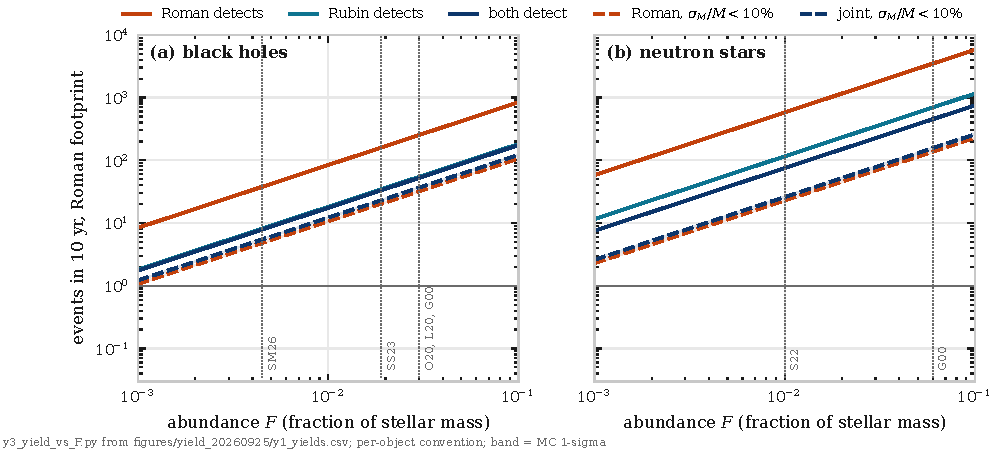
\includegraphics[width=0.9\textwidth]{y3_yield_vs_F}
\caption{Expected footprint events over ten years against the assumed abundance, $N(F)=F\,N_1$;
bands are the Monte Carlo $1\sigma$; dotted verticals mark literature abundances; the horizontal line
is one event.}
\label{fig:yieldF}
\end{figure}

The literature range runs, for black holes, from the $F_{\rm BH}=4$--$5\times10^{-3}$ adopted by
\citet{SajadianMakler2026} to $\approx0.03$, which follows from the $\sim\!10^8$ black holes of
population syntheses (\citealt{Olejak2020}: $1.2\times10^8$ at $\sim\!14\,\Msun$;
\citealt{Lam2020}: $2.2\times10^8$ at $5$--$16\,\Msun$) in a Galaxy of $\sim\!6\times10^{10}\,\Msun$ of stars, and from
the bulge census of \citet{Gould2000}, whose mass
fractions of main-sequence stars, white dwarfs, neutron stars and black holes are $69\!:\!22\!:\!6\!:\!3$;
that census also sets the neutron-star maximum, $F_{\rm NS}=0.06$. \citet{Sweeney2022} put neutron
stars and black holes together at $\sim\!1\%$ of the Galaxy's mass. For $F_{\rm BH}=0.005$--$0.03$, Roman detects
$42$--$252$ black-hole events as simulated, $5$--$32$ of them with a $10\%$ mass; for $F_{\rm NS}=0.005$--$0.06$, $290$--$3{,}480$
neutron-star events and $11$--$137$ masses (Monte Carlo errors $1$--$4\%$ on each). With the dust
corrected (Section~\ref{sec:dust}) these become $28$--$170$ black-hole events and $3$--$17$ masses,
and $180$--$2{,}190$ neutron-star events and $6$--$66$ masses. Only $(66\pm5)\,F$ black-hole
events in the footprint are detected by Rubin and not by Roman, and all of them peak outside Roman's
mission: black-hole events are long enough to overlap a Roman season, and Roman then detects them.
The combination adds $10$--$14\%$ to the number of Roman's $10\%$ masses in every population, while
for the events Rubin detects it turns $8\,F$ black-hole and $0.15\,F$ neutron-star masses into
$(896\pm28)\,F$ and $(1{,}726\pm80)\,F$ (Section~\ref{sec:romanrubin}). Per unit mass, black
holes are poor lenses: the event rate grows only as $\sqrt{\Ml}$ while their number falls as
$1/\Ml$, so at equal $F$ they give far fewer events than neutron stars. They are, however, the
population whose masses are best measured, because a heavy lens gives a large $\tetE$: Roman measures
$60\,F$ black-hole masses to $1\%$, against $12$ ordinary-lens masses (with the dust corrected,
$26\,F$ against $3$). Near the footprint's latitude the model's event rate per star is $25$--$40\%$
below OGLE-IV's (Section~\ref{sec:certainty}), but that comparison was made through the model's
too-thin dust and has to be repeated with the corrected dust before it can say whether the corrected
yields are under- or overstated.

% Source: figures/y2_20260925/y2_ss23.md (counted our way); figures/u7_20260930/u7_ss23_factors.md
% (counted their way; analysis/u7_ss23_factors.py, Deviation 65). Their code:
% github.com/SSajadian54/AstrometryMicrolensing (BH_Roman_V1.cpp, Analyze_IMF1.py).
\paragraph{Against \citet{SajadianSahu2023}.} With their assumptions adopted (their $F_1=0.019$ is our
$F$; their $M^{-1}$ mass function, over $2$--$50\,\Msun$, is our log-uniform one re-weighted to
$3$--$50\,\Msun$), Roman detects $31.5\pm0.5$ black holes per deg$^2$ per season against their $7.3$
($\approx86$ detections over $1.96$\,deg$^2$ and six seasons). Part of the difference is the final
GBTDS design, whose low-cadence seasons fill the gap their forecast assumed. Part is the sample,
as for the fractions below: their count scales the $27{,}000$ detections with $|u_0|<1$ forecast by
\citet{Penny2019}, while ours counts every detection over the decade with $u_0$ up to $3$. Counted our
way -- every Roman detection, weighted by the event rate ($\Neff=4{,}894$) -- the fraction
characterised to $10\%$ is, ours against theirs: $\tetE$ $(88.8\pm0.5)$ against $99.2\%$, $\tE$
$(26.0\pm0.6)$ against $67.0\%$, $\piE$ $(10.0\pm0.4)$ against $30.0\%$, $\Ml$ $(9.3\pm0.4)$ against
$29.8\%$. Their published code counts a different sample: $u_0$ is drawn only up to $1$ (ours to
$3$), $t_0$ only inside Roman's five-year mission (ours across the decade), and events are counted
without the $\sqrt{\Ml}\,v_t$ of the event rate. Of our Roman black-hole detections, $55\%$ have
$u_0>1$ and $36\%$ peak outside Roman's mission, seen on their wings; both are poorly characterised,
and the rate weight favours fast, short events, whose parallax is hardest. Counted their way
($3{,}170$ simulated detections), ours are $\tE$ $(71.9\pm0.8)$ against $67.0\%$, $\piE$
$(42.1\pm0.9)$ against $30.0\%$ and $\Ml$ $(38.1\pm0.9)$ against $29.8\%$. The photometric
forecasts therefore agree, ours somewhat better (their stricter detection cut, not reproduced here,
would if anything raise ours further). The $\sim\!3\times$ shortfall of the first comparison came
from comparing two different samples, not from the forecasts; both codes use the same Roman
photometric error curve. The one real difference left is $\tetE$, $(80.2\pm0.7)$ against $99.2\%$:
their per-exposure astrometric errors, from simulations by S.~Calchi Novati, are $1.6$--$8$ times
smaller than ours over F146\,$=18.5$--$25$, and their astrometric fit holds $\piE$ fixed where ours
fits it.

% =================================================================================================
\FloatBarrier
\subsection{Sample events}
\label{sec:samples}

The results above are statistics over many events. To see individual events, the simulator can
record the full simulated data -- every visit, every band, both observers -- of events chosen by
class. $43$ events were drawn this way, from separate runs of the same model, in the following
classes:

\begin{description}[leftmargin=2.2cm,style=nextline]
\item[\code{both}] detected by Rubin alone and by Roman alone.
\item[\code{roman\_only}] Roman detects, Rubin does not, although Rubin has data near the peak.
\item[\code{rubin\_only}] Rubin detects, Roman does not, although Roman has data within $\pm2\tE$ of
  the peak.
\item[\code{gap\_filler}] Rubin detects, Roman does not, and the peak falls in one of Roman's
  mid-mission gaps at a sightline Roman observes.
\item[\code{astrometric}] detected, with a measurable astrometric signal in Roman's data.
\item[\code{any}, \code{ns\_typical}, \code{bh\_short}, \code{bh\_long}] any joint detection with data
  from both surveys (with $\tE$ cuts for the black-hole classes).
\end{description}

\textbf{The samples illustrate; they are not a representative sample}: they were selected by class
and, for some classes, by tighter cuts. Their precisions are the same Fisher forecasts as in the
statistical results.

\paragraph{How to read a sample figure.} Each is one page with nine panels. The header gives the
true parameters, who detected the event, where the peak falls, and the forecast $1\sigma$ errors
(joint / Rubin / Roman). (a) Magnification over the full ten years, with Roman's seasons shaded
(dark: high cadence); (b) the sky trajectories of source, lens and their separation; (c) magnification
around the peak; (d) the trajectories at closest approach; (e) the per-band light curves in magnitudes;
(f) the parallax signal, data minus the no-parallax model; (g) the centroid shift $|\delta\theta_c|$
against time, with Roman's $1.1$\,mas floor; (h) the centroid ellipse on the sky; (i) the source's and
lens's parallax loops. A point is drawn only if its error is below a third of the signal in that panel.
\emph{``Without parallax'' is the geocentric model} matched to the true trajectory at the peak, the
standard convention \citep{Gould2004}. The $u_{\rm min}$ in a header is the observed closest
approach, and can differ slightly from the tabulated $u_0$.

\paragraph{What the samples show.} Filling the classes was itself informative. The
\code{rubin\_only} class could barely be filled, and every example found (ordinary lenses c001 and
c002; neutron star b001) peaks inside a Roman gap with only two Roman exposures within $\pm2\tE$. For
black holes both Rubin-alone classes stayed \emph{empty}: all $354$ simulated footprint black-hole
events that Rubin detects and Roman does not peak outside Roman's mission, because black-hole events
outlast Roman's gaps. How often ``Rubin alone'' can happen at all depends strongly on the lens
population.

Figures~\ref{fig:s_first}--\ref{fig:s_last} show nine events; all $43$ are tabulated in
Appendix~\ref{app:table} and drawn in Appendix~\ref{app:gallery}. Every figure is a vector PDF and
can be zoomed.

\samplefig{bulge/both/both_008.pdf}{A textbook ordinary event that both surveys detect (ordinary
lenses, \code{both\_008}): $\tE=100$\,d, $u_0=0.13$, a $1\,\Msun$ lens at $6.3$\,kpc, peak in a
Roman gap. $\sigma(\tE)/\tE$ is $0.3\%$ jointly, $2.4\%$ from Rubin alone and $0.4\%$ from Roman
alone; the lens mass is measured to $5.7\%$, essentially by Roman.}{fig:s_first}

\samplefig{bulge/astrometric/astrometric_b003.pdf}{An astrometric example (ordinary lenses,
\code{astrometric\_b003}): a $0.68\,\Msun$ lens at only $0.74$\,kpc gives $\tetE=2.5$\,mas and a
$0.9$\,mas centroid shift, and $\tetE$ is measured to $0.7\%$. The peak falls after Roman's mission.
Roman measures the broad astrometric signal on the wings and Rubin the photometric peak, and together
they bring $\piE$ to $9\%$ and the mass to $9\%$ (Roman alone: $23\%$).}{fig:s_ast}

\samplefig{bulge/gap_filler/gap_filler_012.pdf}{Gap filling (ordinary lenses,
\code{gap\_filler\_012}): a $27$\,d event by a $0.07\,\Msun$ lens, peaking in a mid-mission Roman
gap at a footprint sightline. Roman has two exposures near the peak and does not detect it; Rubin
does. $\sigma(\tE)/\tE$ is $23\%$ jointly against $548\%$ for Roman alone -- the corner where the
gap-filling gain survives.}{fig:s_gap}

\samplefig{bulge/rubin_only/rubin_only_c002.pdf}{A detection by Rubin alone (ordinary lenses,
\code{rubin\_only\_c002}): $\tE=17$\,d, peak magnification $8.5$, in a Roman gap with two Roman
exposures on the wing as the next season opens -- the only way this class arises.}{fig:s_rub}

\samplefig{ns/astrometric/astrometric_001.pdf}{A neutron star weighed (\code{astrometric\_001}):
$1.16\,\Msun$ at $2.0$\,kpc, $\tE=151$\,d, centroid shift $0.52$\,mas; $\tetE$ to $1.3\%$ and the
mass to $1.4\%$ jointly ($1.8\%$ from Roman alone).}{fig:s_nsast}

\samplefig{ns/rubin_only/rubin_only_b001.pdf}{A neutron-star event only Rubin detects
(\code{rubin\_only\_b001}): $\tE=32$\,d, $u_0=0.22$, peak in a gap, two Roman exposures within
$\pm2\tE$. It was the only such event found in a full pass over the footprint.}{fig:s_nsrub}

\samplefig{bh/both/both_011.pdf}{A black hole weighed to half a per cent (\code{both\_011}):
$24\,\Msun$ at $1.9$\,kpc, $\tE=343$\,d, $\tetE=8.5$\,mas, centroid shift $3.0$\,mas. The joint and
Roman-alone precisions are identical ($\tE$ $0.3\%$, $\Ml$ $0.5\%$); Rubin alone gets $\tE$ to
$74\%$.}{fig:s_bh}

\samplefig{bh/astrometric/astrometric_001.pdf}{A very heavy lens (black holes,
\code{astrometric\_001}): $426\,\Msun$ at $6.2$\,kpc, $\tE=838$\,d, $\tetE=16$\,mas, and a centroid
shift of $5.7$\,mas, five times Roman's per-exposure floor. Detected by Roman only; the mass is known
to $30\%$, limited by $\piE$.}{fig:s_bhast}

\samplefig{bh/bh_short/bh_short_b002.pdf}{A short black-hole event (\code{bh\_short\_b002}):
$7.4\,\Msun$ at $9.4$\,kpc, behind the Galactic centre, $\tE=50$\,d. Roman alone gives $\tE$ to
$0.7\%$ and $\tetE$ to $2.2\%$, but the parallax of so distant a lens is small and the mass is known
only to $40\%$ -- the typical limit for black holes.}{fig:s_last}

% =================================================================================================
\section{How certain are these results?}
\label{sec:certainty}

There are two kinds of uncertainty, of very different size: Monte Carlo noise, which is small and
shrinks with more computing, and modelling assumptions, which are larger and do \emph{not} shrink with
more computing. Comparisons with published forecasts test both: the $\sim\!3\times$ disagreement
with \citet{SajadianSahu2023} is explained, and Roman's detection rate is within about a quarter of
\citet{Penny2019}'s (Section~\ref{sec:compare}).

\subsection{Monte Carlo (statistical) uncertainty}
Every number in Section~\ref{sec:results} carries its Monte Carlo $1\sigma$ error. For yields it is
Poisson on the simulated draws; for weighted fractions and medians it is a bootstrap over simulated
events (400 replicates, each re-weighting every event by a Poisson-distributed count), recomputed from
the event tables with the same selections as the original analyses, whose logged values it
reproduces. The yields in Table~\ref{tab:n1} are known to $1$--$2\%$ for Roman's detections, $2$--$4\%$
for Rubin's inside the footprint and $3$--$4\%$ for compact-object $10\%$ masses. The ordinary-lens
selections are the weakest, because the weight concentrates on few events: $13$--$14\%$ for their
$10\%$ masses and $\sim\!30\%$ for their $1\%$ masses ($11.7\pm3.9$). Pooled fractions and medians
are limited by $\Neff$, not by the raw count: $3{,}969$ for the ordinary-lens footprint sample, and
$\sim\!60$--$700$ in the gap-filling bins, so the deepest gap-filling median ($0.08\pm0.06$,
$\Neff=62$) is uncertain by nearly its own size.

\subsection{Checks the results pass}
\begin{table}[h]
\centering
\small
\caption{Independent checks, and what each would have caught.}
\label{tab:checks}
\begin{tabular}{p{0.44\textwidth}p{0.24\textwidth}p{0.22\textwidth}}
\toprule
check & result & would catch \\
\midrule
optical depth from the event-rate constants against direct integration of the density
  & $1.001$ / $1.001$ / $1.000$ (ordinary / black holes / neutron stars) & yield normalisation \\
weighted mean $\tE$ against OGLE-IV \citep{Mroz2019}, $-6^\circ\le b\le-1^\circ$, $|l|<2^\circ$
  & $23.5\pm0.1$ against $23.8\pm0.5$\,d (unweighted: $53.8$\,d) & the event-rate weight \\
$\sigma_{\rm joint}\le\sigma_{\rm single}$, event by event & holds, but for round-off and one
  near-singular event & the three-matrix bookkeeping \\
satellite-parallax control events & median ratio $1.000000$ & the paired L2/Earth design \\
reddening law against published \citet{Cardelli1989} ratios & agrees to $10^{-3}$ & the extinction
  in every band \\
Fisher forecasts against the finite-difference step & on a plateau for every parameter & numerical
  derivatives \\
semi-analytic re-count of resolvable visits against the simulator's own count & same verdict for
  $99.5$--$100\%$ of events & the depth correction of Section~\ref{sec:resolve} \\
\bottomrule
\end{tabular}
\end{table}

\subsection{Modelling uncertainties, ordered by how much they could move the numbers}
\begin{enumerate}
\item \textbf{Roman's $1.1$\,mas astrometric floor is treated as independent between exposures.}
  Every $\tetE$ and lens-mass number for ordinary and neutron-star lenses depends on averaging
  $\sim\!5\times10^4$ exposures down by a factor $\sim\!224$. The floor is a centroiding systematic
  and may be correlated between exposures; in the fully correlated limit most ordinary-lens $\tetE$
  values would be unmeasurable. Black holes are much less affected, since $90\%$ exceed the floor in a
  single exposure. \emph{This is the dominant caveat.} The remedy is a two-component error model,
  with a part that averages down and a correlated part that does not. \citet{Sanderson2019WFIRSTastrometry}
  note that such systematics are often time-dependent ``with unknown correlations'', and quote
  the survey's requirement, as then drafted, of a $10\,\mu$as systematic precision over the full
  survey (stretch goal $3\,\mu$as); they give no split between the two parts, which remains to be
  established.
\item \textbf{The dust is too thin near the Galactic plane.} North of declination $-30^\circ$, which
  includes almost all of Roman's footprint, the extinction tables come from Bayestar, which gives three
  to six times too little extinction within $1^\circ$ of the plane, measured against the independent
  VVV reddening map (Section~\ref{sec:dust}). DECaPS, already in the pipeline, is within $12\%$ of VVV
  farther from the plane but also saturates within $1^\circ$ of it, most of all in the Galactic-centre
  field; there only near-infrared dust is right. The corrected headline numbers are those quoted in
  the abstract and summary; the direction of every Roman--Rubin comparison is unchanged or
  strengthened.
\item \textbf{Roman's photometric error model is provisional}: a tabulated curve not yet checked
  against the F146 noise model of \citet{Wilson2023GBTDS}. Every Roman photometric forecast inherits
  it. Its single-exposure depth in the simulator is a $29$\,mag placeholder, against the curve's own
  $5\sigma$ limit of $25.5$\,mag; this matters for resolving the images, where it has been corrected
  (Section~\ref{sec:resolve}), and hardly for detection ($0.3$--$1\%$ of Roman's detections have
  fainter baselines).
\item \textbf{The event rate is too flat in latitude} compared with OGLE-IV \citep{Mroz2019}: the
  model's rate per star is $1.38$ times the observed one at $b=-5.1^\circ$ and $0.48$ times it at
  $b=-0.1^\circ$, crossing unity near $b=-2.3^\circ$. Full-scan yields carry a systematic of tens of
  per cent; at the footprint's latitude the model is $25$--$40\%$ low. The comparison counts sources
  brighter than $I=21$ as seen through the model's own dust, which is too thin near the plane
  (item~2), so it must be repeated with the corrected dust before its effect on the corrected
  footprint yields is known.
\item \textbf{Mass functions are assumptions}: log-uniform black holes taken as the truth, a single
  Gaussian for neutron stars (the real distribution may be bimodal), and a simple initial--final mass
  relation for the remnants among ordinary lenses. Yields scale with $F$, which is uncertain by an
  order of magnitude; this is why $N_1$ is quoted.
\item \textbf{The GBTDS footprint is a notional layout}, not the adopted one: six fields placed
  with M.\ Penny's field-layout tool and modelled as overlapping circles, $1.47$\,deg$^2$ against
  the design's $1.7$\,deg$^2$, and $\sim\!0.2^\circ$ closer to the plane than the real fields;
  $79\%$ of it lies on real detectors (Fig.~\ref{fig:footreal}). With realistic dust the real
  layout would give Roman $15$--$24\%$ more events (Section~\ref{sec:footunc}). The partial overlap of Rubin's wide pointings with Roman's
  fields is not modelled either, and Roman's start date is a choice (Fig.~\ref{fig:timeline}).
\item \textbf{Resolving the images depends on a criterion no one has calibrated for Roman.} The
  $\mathcal{D}\sigma_a$ bar of \citet{SajadianMakler2026} was built for Rubin's seeing-limited images;
  applied to Roman it sits at a twentieth of the PSF width. The resolvable fractions therefore span two
  orders of magnitude between the permissive and the conservative bar, and only simulated Roman images
  can say where in that range the truth lies.
\item \textbf{The tabulated $t_0$ is not exactly the observed peak} once parallax is included; the
  gap-filling statistics are binned on the peak's distance from a season edge computed from it, which
  is typically off by days.
\item \textbf{Smaller}: Roman's halo orbit about L2 is not modelled; the astrometric shift is not
  diluted by blended light (negligible for Roman); Rubin's astrometric error model is the weakest
  input, but carries no weight in any result.
\end{enumerate}

\subsection{The simulated footprint against the real one}
\label{sec:footunc}

The runs were made on a notional Roman footprint that differs from the adopted one in three ways
(Fig.~\ref{fig:footreal}): it is smaller ($1.47$\,deg$^2$ against $1.71$\,deg$^2$ observed per
season), it sits $\sim\!0.2^\circ$ closer to the Galactic plane, and it ignores that Roman's fields
rotate between the spring and autumn seasons, so that the edges of the real footprint are observed
in only half of them. No run exists on the real layout, but its effect can be estimated from the runs
that do exist, because the simulated footprint spans $0.6^\circ$ in latitude and the yield per
deg$^2$ can be measured row by row across it.

\paragraph{Method.} In each $0.1^\circ$ latitude row of the simulated footprint the yield per deg$^2$
is measured, and $\ln(\text{yield density})$ is fitted as linear in $b$, separately for the five-field
block (six rows) and the Galactic-centre field (six rows). Roman's yield density rises toward the
plane, by $0.7$--$0.9$ per degree in $\ln$ across the five-field block. The fit is then integrated
over the real detector layout, taken separately from the spring and autumn tile images, with each
patch weighted by the fraction of seasons in which it is observed. Its ratio to the same integral
over the simulated cells splits into an area factor and a latitude factor.

% Source: figures/u1_20260929/u3_footprint_offset.csv (analysis/u3_footprint_offset.py) for the
% model's dust, with the 16--84% range from the fit; figures/u1_20260929/u4_dust_check_hybrid.csv
% (analysis/u4_dust_check.py --parts 2 --reference hybrid; Deviation 63) for the corrected dust.
\begin{table}[h]
\centering
\caption{Estimated yield on the real GBTDS layout over the yield on the simulated one. Upper block:
with the model's own dust, which is too thin near the plane (Section~\ref{sec:dust}); in brackets
the $16$--$84\%$ range from the latitude fit. Lower block: with the dust corrected to the reference
of Section~\ref{sec:dust}. Area factor $1.165$ throughout (season-weighted real area over simulated
area); the rest is the latitude dependence.}
\label{tab:footunc}
\small
\begin{tabular}{lccc}
\toprule
 & ordinary lenses & black holes & neutron stars \\
\midrule
\multicolumn{4}{l}{\emph{with the model's dust}} \\
Roman detections                  & $1.05$ ($1.03$--$1.08$) & $1.02$ ($1.01$--$1.04$) & $1.01$ ($0.99$--$1.03$) \\
Roman, $\sigma(\Ml)/\Ml<10\%$     & $1.08$ ($0.94$--$1.22$) & $1.03$ ($1.00$--$1.06$) & $0.95$ ($0.92$--$0.98$) \\
Rubin detections in the footprint & $0.91$ ($0.87$--$0.95$) & $0.99$ ($0.96$--$1.03$) & $0.90$ ($0.88$--$0.93$) \\
\midrule
\multicolumn{4}{l}{\emph{with the dust corrected}} \\
Roman detections                  & $1.24$ & $1.15$ & $1.18$ \\
Rubin detections in the footprint & $2.2$ & $1.8$ & $2.0$ \\
\bottomrule
\end{tabular}
\end{table}

\paragraph{Result.} With the model's own dust the two effects nearly cancel
(Table~\ref{tab:footunc}, upper block). The real fields have $16.5\%$ more area, but in the model
they lie where the event density is $10$--$13\%$ lower for Roman, so Roman's detections would
change by only $+1\%$ to $+5\%$. \textbf{That cancellation is an artefact of the model's dust.} The
model's event density rises toward the plane mainly because its dust there is far too thin: in
front of the bulge at $b=-0.94^\circ$ it has $A_V\approx2.6$, where VVV gives $11.5$ (DECaPS $10.1$),
while at $b=-1.44^\circ$ it has $4.8$, as VVV does (Section~\ref{sec:dust}). With the dust corrected,
Roman's event density across the five-field block is flat in latitude ($-0.14$ to $+0.26$ per degree
in $\ln$, instead of $0.7$--$0.9$), and in the Galactic-centre field it falls toward the plane. The
denser southern sky the simulation missed then more than makes up for the northern rows it included,
and the area and position effects add (lower block): on the real layout Roman detects $15$--$24\%$
more than on the simulated layout with the same corrected dust. Rubin's corrected density falls
steeply toward the plane ($-1.9$ to $-2.6$ per degree in $\ln$ across the five-field block), so on the
real layout, which reaches farther south, it would detect about twice as many events inside the
footprint; this rests on extrapolating that steep fit, and is the least certain number in the
table.
The per-event quantities, the ones most of this report's conclusions rest on, hardly move. Across the
simulated rows the fraction of Roman's detections that it characterises has no measurable latitude
trend in any population, and extrapolated to the real fields' latitude it changes by $1$--$2\%$.
The $10\%$-mass fraction changes by $-10\%$ to $+19\%$, within two standard errors of no change.
The resolvable fraction does have a real trend, rising toward the plane by $\approx3\sigma$ for black
holes and neutron stars, and on the real fields it would be $4$--$12\%$ lower, about $45\%\to44\%$
for Roman's black holes at $\mathcal{D}=5$. These per-event trends were measured with the model's
dust. So the ratios, the gap-filling result, and what each
survey adds to the other carry over to the real layout, and the footprint yields move by less than
their other uncertainties.

\paragraph{What the estimate cannot capture.} It assumes the yield density depends on latitude only
within each block (the real and simulated fields span similar longitudes), and it extrapolates:
$39\%$ of the real five-field area lies south of the last simulated row, and $30\%$ of the real
Galactic-centre field below its own. The exponential fits describe the rows well
($\chi^2$ per degree of freedom $0.2$--$4$; the fit errors are inflated where it exceeds one), but
the extrapolation is untested. The model's
latitude gradient is known to be too flat over the whole bulge (Section~\ref{sec:certainty}, item~4). Within the
footprint's latitudes, however, its departure from OGLE-IV's is consistent with zero
($-0.08\pm0.19$ per degree), and adopting OGLE's gradient shifts the ratios by about $1\%$.
Counting a patch observed in half the seasons as half the yield is an approximation; long events,
which span several seasons, should lose less. The dust correction carries the assumptions listed in
Section~\ref{sec:dust}. Taken together: the corrected dust lowers the simulated footprint's Roman
yields by $33$--$38\%$ (Table~\ref{tab:corrected}), and the real layout then raises them by
$15$--$24\%$, so the real survey should detect $22$--$25\%$ fewer events than the as-simulated Roman
footprint yields of Section~\ref{sec:results}, and $15$--$24\%$ more than the corrected ones of the
abstract. That is larger than their Monte
Carlo errors and far smaller than the uncertainty in $F$. A run on the adopted layout with the right
dust would remove both (Section~\ref{sec:next}).

\subsection{The dust near the Galactic plane: what is wrong and how to correct it}
\label{sec:dust}

Checking the footprint estimate above exposed a larger problem: within about $1^\circ$ of the
Galactic plane the simulation dims its sources by far too little dust. This subsection says what
the simulation does, what is wrong with it and how we know, how much it changes the results, and
what has to be done to correct it.

\paragraph{What the simulation does.} The extinction is pre-computed once per Rubin pointing. For
each, $A_V$ is tabulated against distance out to $20$\,kpc from one of two three-dimensional dust
maps, chosen by declination: Bayestar19 \citep{Green2019Bayestar} north of $-30^\circ$, DECaPS
\citep{Zucker2025DECaPS} south of it, the combination the documentation of the \texttt{dustmaps}
software \citep{Green2018dustmaps} recommends and the DECaPS authors describe. Roman's footprint lies at declination $\approx-29^\circ$, so $139$ of its $147$
sightlines take Bayestar. Each simulated source then takes the table nearest to its sightline, reads
$A_V$ at its own distance, and converts it to every band with the \citet{Cardelli1989} law. We
checked that the simulation did exactly this: the tables match fresh queries of the two maps, and the
extinction recorded for $300{,}000$ simulated sources matches the tables in $99.9\%$ of cases (the
rest are sources equidistant from two tables).

\paragraph{What is wrong.} Each of the two maps fails somewhere, for the same reason: a map built
from stars cannot measure the dust behind which it sees no stars.
\begin{itemize}
\item \emph{Bayestar is used beyond the distance it vouches for.} Bayestar measures dust from stars in
  the optical Pan-STARRS~1 survey, with 2MASS and Gaia \citep{Green2019Bayestar}, and reports, for
  every sightline, the distance out to which that measurement is reliable (a flag returned by
  \texttt{dustmaps}; \citealt{Green2018dustmaps}). On all $139$ of Roman's sightlines that take Bayestar, that flag is false
  beyond $4$\,kpc: toward the inner bulge the dust lanes hide the stars behind them, the map sees the
  dust in front of the lanes and not behind, and its profile goes flat. Every bulge source lies
  beyond that distance. The table-building script requests the flag but does not use it.
\item \emph{DECaPS saturates in the most obscured field.} DECaPS, built from deeper DECam imaging
  together with near-infrared photometry from VVV and 2MASS \citep{Zucker2025DECaPS}, has data at every one of the $1{,}829$ scanned sightlines,
  including the part north of $-30^\circ$ that the declination rule never asks it about, and at
  $8$\,kpc its own flag calls it reliable on all of Roman's five-field block. But it is sensitive
  only up to $A_V\approx12$ \citep{Zucker2025DECaPS}, and toward Roman's Galactic-centre field the
  dust in front of the bulge amounts to $A_V\approx30$. There DECaPS reads $A_V\approx7$, no more than
  it reads a degree farther from the plane, even though its flag is still set on $71\%$ of that
  field's sightlines. Replacing Bayestar by DECaPS everywhere would therefore fix most of the scan,
  but not the Galactic-centre field.
\end{itemize}

The same rule causes a second, smaller fault. Just north of $-30^\circ$ Bayestar's coverage is
ragged, and $78$ of the $2{,}518$ tables came out empty, with no valid value at any distance. The
simulator reads them without checking, and the sightlines that use them were simulated with
essentially no dust at all (median $A_r=0.0002$\,mag, against $\approx3$\,mag elsewhere). There are
$20$ such sightlines, a patch at $l\approx0.1^\circ$--$0.7^\circ$, $b\approx-2.1^\circ$ to $-2.9^\circ$
just south of Roman's footprint, holding $1.3$--$1.7\%$ of all simulated detections. None of them is
in Roman's footprint, so they inflate only Rubin's totals.

\paragraph{How we know.} Choosing between two maps needs a measurement independent of both. We
use the VVV reddening map of \citet{Surot2020}: the $J-K_s$ colour of bulge red-clump and red-giant
stars at a resolution of $2'$ to $10''$, finest near the plane, which measures the whole dust column to the bulge in the near
infrared, where even $A_V\approx30$ does not hide the stars. We took its median in each simulated
sightline's $0.1^\circ$ cell (at least $1{,}600$ grid points per cell) and made two comparisons.

The first needs no extinction law. Each map should reproduce how much more dust lies in front of the
Galactic-centre field than in front of the five-field block, whatever its units. The ratio of the two
columns is $4.89$ for VVV, $4.46$ for the near-infrared map of \citet{Marshall2006} (2MASS $J-K_s$
colours set against the Besan\c{c}on model), $1.07$ for DECaPS and $0.57$ for the simulation's tables. DECaPS misses four fifths of the
Galactic-centre column; the near-infrared map is within $10\%$ of VVV; the simulation's dust even
\emph{decreases} toward the plane, the reverse of the real sky.

The second puts every map on DECaPS's $A_V$ scale, by matching it to DECaPS on the five-field block,
where DECaPS is reliable and far from saturation ($A_{K_s}/A_V=0.0805$ for the near-infrared map,
$E(J-K_s)/A_V=0.133$ for VVV), and compares each with VVV sightline by sightline over the whole scan.
On this scale the Galactic-centre field has $A_V\approx33$ (VVV) and $31$ (near-infrared map) in front
of the bulge, against $7$ (DECaPS) and $2.7$ (the simulation). Across the scan:

% Source: figures/u1_20260929/u6_vvv_scan.csv (analysis/u6_vvv_check.py --scan-log): median over
% sightlines of A_V(8 kpc)/A_V,VVV; A_V,VVV = E(J-Ks)/0.133.
\begin{center}
\small
\begin{tabular}{lccccc}
\toprule
$|b|$ & $0$--$0.5^\circ$ & $0.5$--$1^\circ$ & $1$--$1.5^\circ$ & $1.5$--$2.5^\circ$ & $2.5$--$6^\circ$ \\
\midrule
sightlines                                & $239$ & $215$ & $269$ & $385$ & $721$ \\
$A_V$ in front of the bulge (VVV)         & $24$  & $14$  & $7.6$ & $5.5$ & $2.1$ \\
\midrule
\multicolumn{6}{l}{\emph{ratio to VVV}} \\
the simulation's tables                   & $0.17$ & $0.31$ & $0.88$ & $1.02$ & $1.11$ \\
DECaPS                                    & $0.57$ & $0.86$ & $0.95$ & $0.88$ & $0.89$ \\
near-infrared map                         & $0.98$ & $1.03$ & $1.04$ & $1.11$ & $1.24$ \\
reference used for the correction         & $0.98$ & $0.99$ & $0.96$ & $0.88$ & $0.89$ \\
\bottomrule
\end{tabular}
\end{center}

Within $1^\circ$ of the plane the simulation has three to six times too little dust; farther out it
agrees with VVV to $\sim\!10\%$. DECaPS falls far short only within $1^\circ$ of the plane, where
its sensitivity limit is reached, and is within $12\%$ of VVV elsewhere. The near-infrared map is
right near the plane and gives $11$--$24\%$ more dust than VVV far from it.

\paragraph{Corrected results.} Extra dust only makes a source fainter, so its effect can be estimated
from the draws that exist. The reference dust is the combination the table above supports: DECaPS out
to the distance its own flag calls reliable, and the near-infrared map on DECaPS's scale from the
distance at which it passes DECaPS's limit of $A_V=12$. It follows VVV to within $12\%$ in every
latitude band (last row of the table), and it switches to the near-infrared map before $8$\,kpc on
$444$ of the $1{,}829$ sightlines, $403$ of them within $1^\circ$ of the plane and none beyond
$2.2^\circ$. For every
simulated source the difference between the reference and the simulation's extinction is taken at the
source's own distance, and the source is dimmed by it ($A_{\rm F146}=0.197\,A_V$, $A_r=0.854\,A_V$,
the simulation's own conversion). The probability of each outcome -- detection by Roman or Rubin, a
mass to $10\%$, a characterised event -- is measured from the same draws as a function of magnitude,
and each event is re-weighted by how that probability changes at its dimmed magnitude. Rubin's
probabilities are measured separately for sightlines with different numbers of Rubin visits; the
two-image resolution count is redone visit by visit with the dimmed magnitudes. With no extra dust the
procedure reproduces every number of Section~\ref{sec:results} exactly.

Each corrected number carries two errors. The Monte Carlo error comes from the finite number of
draws. The correction's own systematic error adds in quadrature the shift of its result under three
changes:
\begin{itemize}
\item the near-infrared map used at every distance, instead of DECaPS;
\item the near-infrared map converted with $A_{K_s}/A_V=0.0734$ instead of $0.0805$, which raises
  its column by the $10\%$ by which its Galactic-centre contrast falls short of VVV's (the nominal
  Galactic-centre column is $5\%$ below VVV's, this one $4\%$ above), or with $0.102$, the
  \citet{Cardelli1989} value for $K$ ($2.2\,\mu$m) at the $R_V=2.5$ that the simulation itself uses
  (the larger of the two shifts);
\item the efficiencies measured over the whole footprint, instead of per field block.
\end{itemize}
DECaPS alone is not counted as an alternative, because VVV rules it out in the Galactic-centre field.
Table~\ref{tab:corrected} gives the headline numbers; the abstract and the summary quote the corrected
ones.

% Source: figures/u1_20260929/u5_corrected_numbers.{md,csv} (analysis/u5_corrected_numbers.py,
% Deviation 63). Each cell: as simulated -> dust-corrected +- (Monte Carlo (+) correction systematic).
\begin{table}[h]
\centering
\caption{Headline numbers as simulated $\to$ with the dust corrected, $\pm$ the total $1\sigma$
uncertainty of the corrected value (Monte Carlo and correction systematic in quadrature). Yields
$N_1$ are per unit abundance (ordinary lenses: $F=1$) over ten years; ``footprint'' is Roman's
simulated footprint. Roman's resolution figures are at its $5\sigma$ single-exposure depth
(Section~\ref{sec:resolve}). Centroid shifts and $A_V$ are medians over Roman's footprint
detections.}
\label{tab:corrected}
\footnotesize
\setlength{\tabcolsep}{2pt}
\begin{tabular}{lccc}
\toprule
 & ordinary lenses & black holes & neutron stars \\
\midrule
Roman detections, $N_1$ [$10^3$] & $81.9\to50.4\pm2.9$ & $8.40\to5.66\pm0.32$ & $57.9\to36.5\pm2.3$ \\
Roman, $\sigma(\Ml)/\Ml<10\%$, $N_1$ & $1930\to830\pm110$ & $1068\to579\pm42$ & $2286\to1102\pm72$ \\
Roman, $\sigma(\Ml)/\Ml<1\%$, $N_1$ & $11.7\to3.2\pm2.0$ & $59.8\to25.9\pm3.9$ & $40.5\to20.4\pm3.3$ \\
joint over Roman, $\sigma(\Ml)/\Ml<10\%$ & $1.10\to1.09\pm0.03$ & $1.14\to1.13\pm0.02$ & $1.14\to1.13\pm0.02$ \\
Rubin, footprint, $N_1$ [$10^3$] & $16.8\to4.9\pm0.5$ & $1.81\to0.69\pm0.07$ & $11.6\to3.6\pm0.4$ \\
Rubin, whole scan, $N_1$ [$10^3$] & $175\to78\pm12$ & $24.3\to11.2\pm1.5$ & $141\to62\pm9$ \\
detections outside footprint [\%] & $63.8\to58.5\pm5.1$ & $72.7\to65.0\pm4.1$ & $67.5\to60.9\pm4.7$ \\
\midrule
\multicolumn{4}{l}{\emph{Rubin's footprint detections, Rubin alone / joint (Section~\ref{sec:romanrubin})}} \\
characterised [\%] & $4.6\pm1.4$ / $28.2\pm2.5$ & $11.9\pm1.1$ / $82.9\pm1.4$ & $4.8\pm0.4$ / $37.2\pm1.6$ \\
$\Ml$ to $10\%$, joint [\%] & $8.9\to8.1\pm1.5$ & $49.5\to53.3\pm1.8$ & $14.9\to15.7\pm1.2$ \\
median $\sigma_{\rm joint}/\sigma_{\rm Rubin}$, $\tE$ & $0.157\to0.097\pm0.020$ & $0.065\to0.059\pm0.003$ & $0.132\to0.133\pm0.023$ \\
\midrule
median $\sigma_{\rm joint}/\sigma_{\rm Roman}$, $\tE$ & $0.9988\to0.9988\pm0.0002$ & $0.9971\to0.9965\pm0.0005$ & $0.9989\to0.9988\pm0.0001$ \\
median centroid shift [mas] & $0.125\to0.123\pm0.002$ & $3.38\to3.39\pm0.04$ & $0.254\to0.252\pm0.002$ \\
$P$(resolvable), Roman, $\mathcal{D}=5$ [\%] & $1.4\to0.8\pm0.3$ & $45.4\to34.2\pm1.2$ & $2.9\to1.7\pm0.2$ \\
\quad $\mathcal{D}=20$ / PSF width [\%] & $<0.001$ / $0$ & $15.3\pm0.9$ / $0.25\pm0.04$ & $0.017\pm0.006$ / $<10^{-4}$ \\
median $A_V$, Roman's detections & $3.6\to7.2\pm0.3$ & $4.2\to7.5\pm0.4$ & $3.7\to7.3\pm0.3$ \\
\bottomrule
\end{tabular}
\end{table}

\paragraph{What it does to the conclusions.} Absolute yields drop, Rubin's more than Roman's, because
the extra dust costs $4.3$ times more in $r$ than in F146. Roman's footprint detections fall by
$33$--$38\%$ and its $10\%$ masses by $46$--$57\%$; Rubin's footprint detections fall by $62$--$71\%$
and its whole-scan detections by $54$--$56\%$. Inside the footprint Roman now detects ten times as many
ordinary-lens events as Rubin, instead of five. The per-event results barely move. The share of
Rubin's footprint events that Roman makes characterisable is unchanged or larger ($28$, $83$ and
$37\%$), and the share with a $10\%$ mass moves by less than four percentage points ($8.9\to8.1\%$,
$49.5\to53.3\%$ and $14.9\to15.7\%$ for ordinary lenses, black holes and neutron stars). Roman sharpens
Rubin's timescales by more than before (a median ten-fold for ordinary lenses, instead of six-fold).
What Rubin adds to Roman's events is still under $0.4\%$ in timescale precision and at most
$9$--$13\%$ in the number of $10\%$ masses, and the centroid shifts are unchanged. Every comparison between the
surveys therefore survives, and those in Roman's favour strengthen. The one gain in Rubin's favour
inside the footprint, gap filling (Section~\ref{sec:gap}), could not be corrected this way and can
only shrink. The fractions of Roman's detections whose two images are resolvable at
$\mathcal{D}=5$ fall by a quarter for black holes ($45\to34\%$) and by $42$--$43\%$ for neutron
stars and ordinary lenses.

\paragraph{Limits of the estimate.} The correction assumes that dimming a source changes an event's
outcomes only through the source's magnitude, with the probability of each outcome measured within a
field block or visit class. Fractions are ratios of corrected yields, each outcome with its own
probability, so they include the loss of precision; but for the medians of per-event ratios, events
are re-weighted only by whether they are still detected, so any further loss of precision in the
survivors is not included, and the joint $10\%$ masses are re-weighted with Roman's magnitude alone. That loss falls mostly on Rubin, whose
sources are dimmed $4.3$ times as much, so the medians of $\sigma_{\rm joint}/\sigma_{\rm Rubin}$
understate Roman's gain for Rubin, and what Rubin adds to Roman (the $<0.4\%$ in timescale, the
$9$--$13\%$ in $10\%$ masses, and gap filling) are upper limits. The
near-infrared map has a resolution of $15'$, so where it is used it smooths over the patchiness of the
Galactic-centre dust; its median agrees with VVV's to $5\%$ there, but the spread between sightlines
is not captured. Where DECaPS is used, its $A_V$ is converted to F146 and $r$ with the simulation's own
\citet{Cardelli1989} law at $R_V=2.5$, whose uncertainty is not included. Far from the plane the
reference follows DECaPS, which has $11\%$ less dust than VVV there, while the simulation's own dust
is within $2$--$11\%$ above it; the correction there therefore brightens the sources slightly, an
effect the near-infrared variant bounds from the other side. The Rubin resolution figures of
Section~\ref{sec:resolve} were not corrected. The numbers in Table~\ref{tab:corrected} are therefore
best estimates with stated errors, not a replacement for a simulation with the right dust.

\paragraph{How to correct it.} No new survey data are needed: DECaPS and the near-infrared map are
already available through the same software the pipeline uses, and together they reproduce VVV
(last row of the table above). What has to change, and what does not:
\begin{itemize}
\item \emph{The table-building script} (\texttt{maps.py}) must change; it is the fault.
\item \emph{The table reader} (\texttt{readBayestar}) must change, to refuse bad tables; this is a
  safeguard, not physics.
\item \emph{The simulator's physics does not change}: the way a source is dimmed, $A_V$ at its distance
  converted to each band, is not at fault.
\item \emph{New production runs are needed}, because the simulator reads the tables and dims every
  source as it runs, so no change to the tables reaches the results without re-running. The
  corrected numbers above stand in until then.
\end{itemize}
The steps, in order:
\begin{enumerate}
\item \emph{Rebuild every extinction table from the reference used for the correction.} Take DECaPS
  for every sightline, dropping the declination rule. Keep DECaPS out to the distance its own flag
  calls reliable, and beyond that add the near-infrared map's further increase. From the distance at
  which the near-infrared map, put on DECaPS's scale ($A_{K_s}/A_V=0.0805$), reaches DECaPS's limit of
  $A_V=12$, take the near-infrared map itself. Bayestar is then needed only where DECaPS has no data,
  which in this scan is nowhere, and only within its own reliable distance. This also removes the $78$
  empty tables. The code that computed the correction already implements this rule, so it can be
  reused as it stands.
\item \emph{Make the pipeline refuse bad tables instead of using them.} The table-building script
  should stop on any table with a missing value rather than print a note. The simulator should check
  every value it reads and refuse a table that fails to parse or holds a non-number, instead of
  continuing silently with no dust.
\item \emph{Check the new tables against VVV before any run.} Repeat this section's comparison on
  the new tables. The ratio to VVV should be $0.9$--$1.0$ in every latitude band (it is now $0.17$ in
  the band nearest the plane), with no fall toward the plane, and the Galactic-centre to five-field
  contrast should be $\approx4.5$--$4.9$ (now $0.57$). Then run a short pilot and confirm that the
  extinction the simulated sources receive matches the new tables.
\item \emph{Re-run the three production runs}, together with the other fixes that need new runs
  (Roman's single-exposure depth, the scan's corner cut, the adopted GBTDS layout), so that the runs
  are repeated once. The new yields should then agree with the corrected numbers above within their
  errors; if they do not, the efficiency-based estimate is missing something and should be understood
  before the results are used.
\end{enumerate}
A further refinement, not needed for the fix: where the near-infrared map is used, F146 could be
derived from $A_{K_s}$ with a near-infrared extinction law, instead of through $A_V$ and the
\citet{Cardelli1989} law.

\subsection{Comparisons with published forecasts}
\label{sec:compare}
% Source: Roman detections per deg^2 of footprint per day of Roman coverage (693 d):
% 81,860 / (1.47 x 693) as simulated, 50,350 +- 2,945 / (1.47 x 693) dust-corrected
% (figures/u1_20260929/u5_corrected_numbers.md); Penny et al. 2019 Table 2 and Sec. 2 ("we can
% expect to detect ~27,000 microlensing events with |u0| < 1 and roughly twice this with |u0| < 3"):
% both figures are DETECTIONS, so ours (u0 <= 3) compares with the second; there is no bracket
% (corrected 2026-09-30, Deviation 66).
\begin{itemize}
\item \textbf{Roman's detection rate is within about a quarter of \citet{Penny2019}'s.} They forecast
  that Roman will detect $\sim\!27{,}000$ events with $|u_0|<1$ and roughly twice that with
  $|u_0|<3$, over $1.96$\,deg$^2$ and six $72$-day seasons: $31.9$ and $63.8$ per deg$^2$ per day of
  coverage. Both are detections, and ours, with $u_0$ drawn up to $3$, compares with the second. As
  simulated it is $80.4\pm1.4$, $(26\pm2)\%$ above it; with the dust corrected it is $49.4\pm2.9$,
  $(23\pm5)\%$ below it, so the correction turns an excess into a shortfall of similar size. The two
  figures are not like for like: ours spreads over ten seasons, four of them low-cadence, and
  includes events that peak outside the seasons, and the detection criterion, the field layout and
  the source counts differ too. None of these differences has been quantified.
\item \textbf{Roman's black-hole characterisation agrees with \citet{SajadianSahu2023}} once their
  sample is reproduced (Section~\ref{sec:yield}). Their fractions are of events with $u_0<1$ peaking
  inside Roman's mission, counted without the event-rate weight; counted that way ours are
  $1.1$--$1.4$ times theirs for $\tE$, $\piE$ and the mass, against $\sim\!1/3$ when every detection
  is counted and weighted by the rate. The remaining difference, $\tetE$ ($0.8$ times theirs), is in
  the direction of two known differences, their $1.6$--$8$ times smaller per-exposure astrometric
  errors and their simpler astrometric fit; how much each contributes has not been tested.
\end{itemize}

\subsection{Summary: what to believe}
\begin{center}
\small
\begin{tabular}{p{0.52\textwidth}p{0.12\textwidth}p{0.28\textwidth}}
\toprule
result & confidence & main risk \\
\midrule
Roman dominates inside its footprint; Rubin adds $<0.4\%$ there & high & Roman photometric error
  model \\
Roman turns Rubin's footprint detections into measurements ($6$--$8\times$ more characterised; masses
  from $\sim\!0$ to $8$--$53\%$) & high & Roman photometric error model; astrometric floor \\
about $60\%$ of detections are outside the footprint, Rubin's alone & high & latitude gradient \\
gap filling only deep in gaps, for short events, an order of magnitude & medium & $\Neff=62$; $t_0$
  offset; not dust-corrected (an upper limit) \\
satellite parallax $<1\%$ pooled & high & halo orbit (small) \\
$\tetE$ is Roman's measurement; black-hole $\tetE$ robust & high (bh) & -- \\
ordinary and neutron-star $\tetE$ and masses & medium--low & correlated astrometric floor \\
absolute yields $N_1$ & medium--low & dust near the plane (corrected, $-33$ to $-71\%$); latitude
  gradient, to be re-measured with the corrected dust \\
yields $N(F)$ & low & $F$ unknown to $\times10$ \\
$\piE$ and mass fractions agree with Sajadian \& Sahu on their sample & medium & sample definition;
  astrometric error model ($\tetE$) \\
resolving the images: black holes $0.3$--$34\%$ (Roman), others rare & low & the resolution criterion
  for Roman \\
\bottomrule
\end{tabular}
\end{center}

% =================================================================================================
\section{Summary}
\label{sec:summary}

\begin{enumerate}
\item \textbf{Roman is the survey inside its footprint.} Over the decade it detects
  $(5.04\pm0.29)\times10^4$ ordinary-lens events there, ten times Rubin's, and measures
  $830\pm110$ lens masses to $10\%$. Dust is the main reason: at the median extinction of
  Roman's footprint detections, $A_V=7.2\pm0.3$, F146 loses $1.4$\,mag where $r$ loses $6.1$.
\item \textbf{Roman transforms the events Rubin detects inside its footprint.} Adding Roman's data
  characterises $6$--$8$ times as many of them, sharpens their timescales a median $8$--$17$-fold,
  and gives lens masses to $10\%$ for $8\%$ (ordinary lenses), $16\%$ (neutron stars) and $53\%$
  (black holes) of them, where Rubin alone gives essentially none. The reverse gain is at most
  $9$--$13\%$.
\item \textbf{Rubin is the survey everywhere else}, supplying $(58.5\pm5.1)\%$ of all detections from
  outside Roman's footprint, and inside the footprint it matters only for short events that fall
  wholly inside Roman's gaps, where it improves $\sigma(\tE)$ by an order of magnitude as simulated;
  this gain is not dust-corrected, and the corrected dust can only reduce it.
\item \textbf{Roman's ten seasons give the parallax of long events on their own}; Rubin's
  longer baseline adds $<0.4\%$ even for multi-year black-hole events. Roman at L2 adds $<1\%$.
\item \textbf{The combination} characterises events neither survey can alone and adds at most
  $9$--$13\%$ to the number of Roman's $10\%$ mass measurements.
\item \textbf{Compact objects.} Roman detects $(5{,}660\pm320)\,F$ black-hole events and
  $(36{,}500\pm2{,}300)\,F$ neutron-star events, measuring $(579\pm42)\,F$ and $(1{,}102\pm72)\,F$
  masses to $10\%$; at $F_{\rm BH}=0.01$ that is $57$ events and $6$ masses. Black-hole Einstein
  radii are measured in single exposures; their masses are limited by the parallax.
\item \textbf{The two images of a black-hole lens are often resolvable in principle.} Roman separates
  them in $0.3$--$34\%$ of its black-hole detections depending on the criterion, and Rubin in about
  $5\%$ of its own at the most permissive one; for lighter lenses resolution is rare.
\item \textbf{The astrometric masses of ordinary lenses and neutron stars rest on one assumption}:
  that Roman's centroiding floor averages down over $5\times10^4$ exposures.
\item \textbf{The yields, fractions and medians here are corrected for the model's too-thin dust
  near the plane} (Table~\ref{tab:corrected}), with a reference dust checked against the independent
  VVV reddening map. The gap-filling gain is as simulated, and the corrected dust can only lower it;
  Rubin's resolution figure is also as simulated. With the dust corrected, Roman's detection rate
  is $(23\pm5)\%$ below \citet{Penny2019}'s forecast for the same range of $u_0$, where as simulated
  it was $26\%$ above it; the survey designs differ in ways not yet quantified. The correction lowered Roman's footprint yields by $33$--$38\%$ (its $10\%$ masses by
  $46$--$57\%$) and Rubin's by $54$--$71\%$, and left the comparisons between the surveys intact or
  strengthened. The proper fix is to rebuild the extinction tables from DECaPS, with near-infrared dust
  where DECaPS saturates, within $\sim\!1^\circ$ of the plane, and re-run; the adopted GBTDS layout
  would then add $15$--$24\%$ to Roman's yields.
\end{enumerate}

% =================================================================================================
\section{Next steps}
\label{sec:next}

The work ahead has two parts: a much finer simulation of Roman's footprint, and the model
improvements that should come before it. Fig.~\ref{fig:roadmap} shows the intended order.

\begin{figure}[h]
\centering
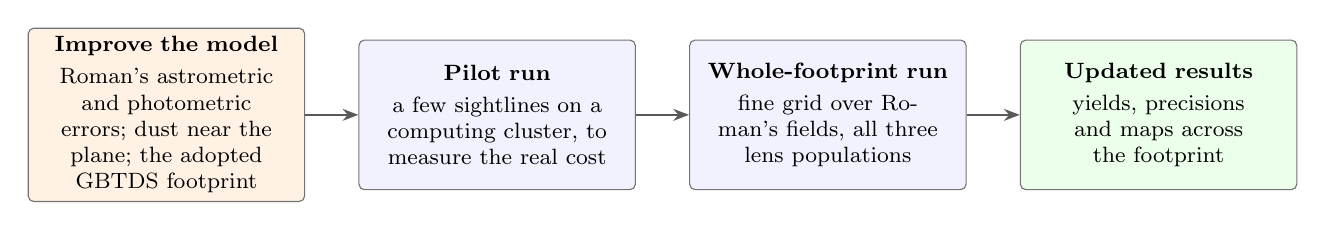
\begin{tikzpicture}
\node[box, fill=orange!10, text width=3.3cm, minimum height=1.9cm] (m) at (0,0)
  {\textbf{Improve the model}\\[2pt] Roman's astrometric and photometric errors; dust near the
   plane; the adopted GBTDS footprint};
\node[box, text width=3.3cm, minimum height=1.9cm] (p) at (4.2,0)
  {\textbf{Pilot run}\\[2pt] a few sightlines on a computing cluster, to measure the real cost};
\node[box, text width=3.3cm, minimum height=1.9cm] (f) at (8.4,0)
  {\textbf{Whole-footprint run}\\[2pt] fine grid over Roman's fields, all three lens populations};
\node[box, fill=green!8, text width=3.3cm, minimum height=1.9cm] (r) at (12.6,0)
  {\textbf{Updated results}\\[2pt] yields, precisions and maps across the footprint};
\draw[arr] (m) -- (p);
\draw[arr] (p) -- (f);
\draw[arr] (f) -- (r);
\end{tikzpicture}
\caption{The intended order of the next steps. The model comes first because more computing
reduces only the Monte Carlo noise, while the model changes the numbers themselves.}
\label{fig:roadmap}
\end{figure}

\subsection{Simulating the whole footprint at full resolution}
The present runs sample Roman's footprint on a $0.1^\circ$ grid of $147$ sightlines, each standing
for $0.01$\,deg$^2$. The natural next step is to cover the whole footprint finely, down to a
$0.02^\circ$ grid of about $3{,}700$ sightlines, for all three lens populations. This would bring:
\begin{itemize}
\item \textbf{Precision where the results are thinnest.} About $25$ times the footprint statistics,
  so Monte Carlo errors about five times smaller. The quantities that gain most are the most
  interesting ones: the gap-filling gain for short events deep inside Roman's gaps (now resting on
  $\Neff=62$), the yields of lens masses measured to $1\%$ and $5\%$ (the $1\%$ yield of ordinary
  lenses is currently uncertain by $\sim\!30\%$), the rare events only Rubin detects inside the
  footprint, and the long-timescale tail of black-hole events.
\item \textbf{Maps instead of averages.} Stellar density and dust vary across Roman's fields, most
  of all toward the Galactic-centre field, and the yields and precisions vary with them. The present
  grid resolves this only coarsely. A fine one would show where in the footprint the most events and
  the best-measured masses are, and whether there are patches where the dust is thin enough for
  Rubin to contribute more.
\item \textbf{A sharper comparison with the literature.} With the footprint finely sampled, the
  yield can be restricted to the fields, seasons and impact parameters that \citet{Penny2019}
  simulated, which would make the comparison with their detection rate like for like and locate the
  remaining $\sim\!25\%$ difference.
\end{itemize}

What it would \emph{not} bring is a change in any result in expectation: a larger run shrinks the
error bars around the same numbers, so every conclusion in Section~\ref{sec:results} should survive
it.

\paragraph{The challenges.}
\begin{itemize}
\item \textbf{Computing time.} The present runs took $16$--$27$ processor-hours per population. The
  finest grid needs roughly $10$--$20$ times as much, a few hundred processor-hours each, which
  means a computing cluster rather than a single machine. The exact cost is uncertain, which is what
  the pilot run is for.
\item \textbf{Splitting the work honestly.} On a cluster the sky is divided into many pieces run in
  parallel. Each piece needs its own independent stream of random numbers -- otherwise the pieces
  would repeat one another's random draws and the error bars would be too small -- and the pieces
  have to be recombined and checked against an undivided run. The simulator needs small additions
  for this, not yet made.
\item \textbf{Getting the order right.} Because computing does not touch the modelling, the model
  improvements below should come first; a whole-footprint run made before them would have to be
  repeated. In particular the run should use the adopted GBTDS footprint rather than the older
  design, and extinction tables rebuilt from DECaPS, with near-infrared dust where DECaPS saturates.
\end{itemize}

\subsection{The most important open items}
These are the known limitations that most affect the results, roughly in order of their impact
(Section~\ref{sec:certainty} gives their current size).
\begin{enumerate}
\item \textbf{Roman's astrometric error.} Whether the $1.1$\,mas centroiding floor averages down
  over $5\times10^4$ exposures decides whether the Einstein radii, and so the masses, of ordinary
  lenses and neutron stars are measurable at all. The plan is a two-component error model, with a
  correlated part that does not average down. The published work gives no split between the two
  parts, only the survey's $10\,\mu$as systematic requirement \citep{Sanderson2019WFIRSTastrometry}, so
  the split has to be established, from simulated Roman images or from the Roman project.
\item \textbf{The dust near the plane.} A declination rule gives almost all of Roman's footprint to
  Bayestar, which cannot see stars behind the dust lanes and gives three to six times too little
  extinction within $1^\circ$ of the plane, measured against the independent VVV reddening map
  (Section~\ref{sec:dust}). The extinction tables should be rebuilt from DECaPS, which the pipeline
  already uses and which covers the whole scan, with near-infrared dust \citep{Marshall2006} where
  DECaPS saturates, within $\sim\!1^\circ$ of the plane; then checked against VVV and the runs
  repeated. The four steps are listed at the end of Section~\ref{sec:dust}. This moves the absolute
  yields by $33$--$71\%$, more than any other open item except the astrometric floor.
\item \textbf{Roman's photometric noise.} The present tabulated curve should be replaced by a
  noise model derived from simulated GBTDS images \citep{Wilson2023GBTDS}; every Roman photometric
  forecast depends on it.
\item \textbf{The survey geometry.} The simulated footprint is a notional six-field layout,
  modelled as overlapping circles ($1.47$\,deg$^2$ instead of $1.7$) and placed $\sim\!0.2^\circ$
  closer to the plane than the real fields (Fig.~\ref{fig:footreal}). It should be replaced by the
  adopted GBTDS fields, with Rubin's larger fields that only partly overlap Roman's handled
  properly, and Roman's start date revisited.
\item \textbf{The event rate's latitude dependence.} The Galactic model's event rate is too flat in
  latitude compared with OGLE-IV. This sets the absolute yields. The comparison was made through the
  model's too-thin dust, so it has to be repeated with the corrected dust first.
\item \textbf{The lens mass functions.} The remnants among ordinary lenses use a simple
  initial--final mass relation, the neutron stars a single Gaussian where the real distribution may
  be bimodal, and the black holes a log-uniform prior. These are scientific choices as much as
  technical ones.
\item \textbf{An external check of Rubin's results.} The Rubin-only forecasts have no independent
  check yet: the closest published study \citep{Abrams2025MicrolensingRubin} quotes no directly
  comparable number, so the check means running their method on the same cadence as ours.
\item \textbf{Detections from the wings.} $3$--$4.4\%$ of Roman's detections have no Roman data
  within $\pm2\tE$ of the peak: a long, slow brightening seen only on its wing, over tens of thousands
  of exposures. A real survey fits the baseline, and such a slow wing is partly degenerate with it, so
  whether to count these events is a convention still to be decided. It moves the yields by at most
  $4.4\%$.
\end{enumerate}

% =================================================================================================
\appendix

\section{All sample events}
\label{app:table}

\scriptsize\setlength{\tabcolsep}{2.5pt}
\begin{longtable}{llrrrrlrrp{1.9cm}p{1.2cm}l}
\caption{Every sample event. Pop.: lens population (bulge = ordinary lenses). Det.: which survey
detects it alone (L = Rubin, R = Roman). Peak: where $t_0$ falls (in a Roman season / in a
mid-mission gap / outside Roman's mission). Shift: maximum centroid shift [mas]. Precisions in per
cent, joint (J), Rubin (L) and Roman (R); n/m = not measured. The verdict is how well the event
illustrates its class.}\\
\toprule
pop. & event & $\tE$\,[d] & $u_0$ & $\Ml$\,[$\Msun$] & $D_L$\,[kpc] & det. & peak & shift & $\sigma_{\tE}/\tE$ J/L/R & $\sigma_M/M$ J/R & verdict \\
\midrule
\endfirsthead
\toprule
pop. & event & $\tE$ & $u_0$ & $\Ml$ & $D_L$ & det. & peak & shift & $\sigma_{\tE}/\tE$ J/L/R & $\sigma_M/M$ J/R & verdict \\
\midrule
\endhead
\sampletable
\end{longtable}
\normalsize

\clearpage
\section{Sample gallery}
\label{app:gallery}

The remaining sample events, three to a row, in the order of the table in Appendix~\ref{app:table}
(the nine events of Section~\ref{sec:samples} are not repeated). The figures are vector graphics and
can be zoomed.

\newcommand{\gal}[2]{\begin{subfigure}[t]{0.32\textwidth}\centering
  \includegraphics[width=\linewidth]{#1}\caption*{\scriptsize #2}\end{subfigure}}

\begin{figure}[!htb]\centering
\gal{bulge/any/any_005.pdf}{bulge any\_005}\hfill
\gal{bulge/any/any_006.pdf}{bulge any\_006}\hfill
\gal{bulge/astrometric/astrometric_001.pdf}{bulge astrometric\_001}\\[4pt]
\gal{bulge/astrometric/astrometric_002.pdf}{bulge astrometric\_002}\hfill
\gal{bulge/astrometric/astrometric_b001.pdf}{bulge astrometric\_b001}\hfill
\gal{bulge/astrometric/astrometric_b002.pdf}{bulge astrometric\_b002}
\caption{Ordinary lenses (1/3).}\end{figure}

\begin{figure}[!htb]\centering
\gal{bulge/both/both_007.pdf}{bulge both\_007}\hfill
\gal{bulge/both/both_009.pdf}{bulge both\_009}\hfill
\gal{bulge/gap_filler/gap_filler_010.pdf}{bulge gap\_filler\_010}\\[4pt]
\gal{bulge/gap_filler/gap_filler_011.pdf}{bulge gap\_filler\_011}\hfill
\gal{bulge/roman_only/roman_only_003.pdf}{bulge roman\_only\_003}\hfill
\gal{bulge/roman_only/roman_only_004.pdf}{bulge roman\_only\_004}
\caption{Ordinary lenses (2/3).}\end{figure}

\begin{figure}[!htb]\centering
\gal{bulge/rubin_only/rubin_only_c001.pdf}{bulge rubin\_only\_c001}\hfill
\gal{ns/astrometric/astrometric_002.pdf}{ns astrometric\_002}\hfill
\gal{ns/both/both_008.pdf}{ns both\_008}\\[4pt]
\gal{ns/both/both_009.pdf}{ns both\_009}\hfill
\gal{ns/both/both_010.pdf}{ns both\_010}\hfill
\gal{ns/gap_filler/gap_filler_011.pdf}{ns gap\_filler\_011}
\caption{Ordinary lenses (3/3) and neutron stars (1/2).}\end{figure}

\begin{figure}[!htb]\centering
\gal{ns/gap_filler/gap_filler_012.pdf}{ns gap\_filler\_012}\hfill
\gal{ns/ns_typical/ns_typical_004.pdf}{ns ns\_typical\_004}\hfill
\gal{ns/ns_typical/ns_typical_006.pdf}{ns ns\_typical\_006}\\[4pt]
\gal{ns/ns_typical/ns_typical_007.pdf}{ns ns\_typical\_007}\hfill
\gal{ns/roman_only/roman_only_003.pdf}{ns roman\_only\_003}\hfill
\gal{ns/roman_only/roman_only_005.pdf}{ns roman\_only\_005}
\caption{Neutron stars (2/2).}\end{figure}

\begin{figure}[!htb]\centering
\gal{bh/astrometric/astrometric_005.pdf}{bh astrometric\_005}\hfill
\gal{bh/bh_long/bh_long_009.pdf}{bh bh\_long\_009}\hfill
\gal{bh/bh_long/bh_long_010.pdf}{bh bh\_long\_010}\\[4pt]
\gal{bh/bh_short/bh_short_004.pdf}{bh bh\_short\_004}\hfill
\gal{bh/bh_short/bh_short_008.pdf}{bh bh\_short\_008}\hfill
\gal{bh/bh_short/bh_short_b001.pdf}{bh bh\_short\_b001}
\caption{Black holes (1/2).}\end{figure}

\begin{figure}[!htb]\centering
\gal{bh/both/both_006.pdf}{bh both\_006}\hfill
\gal{bh/both/both_007.pdf}{bh both\_007}\hfill
\gal{bh/roman_only/roman_only_002.pdf}{bh roman\_only\_002}\\[4pt]
\gal{bh/roman_only/roman_only_003.pdf}{bh roman\_only\_003}\hfill
\mbox{}\hfill\mbox{}
\caption{Black holes (2/2).}\end{figure}

\bibliographystyle{plainnat}
\bibliography{../refs}

\end{document}
